\chapter{Evaluierung}



\section{Strommessung}

Zur Qualitätsbewertung der Strommessung wurde das Fahrzeug aufgebockt. 
Das Fahrzeug befand sich während aller Messungen im Akkubetrieb, bei ca. \SI{16,8}{\volt} Akkuspannung.
Während aller Messungen im Akkubetrieb wurden zwei Akkus parallel genutzt um den Innenwiderstand zu verringern.
Der Motor wurde, soweit nicht anders beschrieben, mit einem PWM-Tastgrad von 30:256 angesteuert.
Zur Beurteilung der Messergebnisse wurden Messungen an diversen Punkten vorgenommen und mit der Ausgabe des Mikrocontrollers verglichen.

Zuerst wurde dazu die Spannung direkt am Shuntwiderstand gemessen.
Dabei kann der periodische Anstieg der Spannung am Shunt beobachtet werden, zu sehen in \cref{fig:filter_eingang}. Die Spannung am Shunt ist proportional zum Strom durch den Motor.

\begin{figure}[H]
\centering
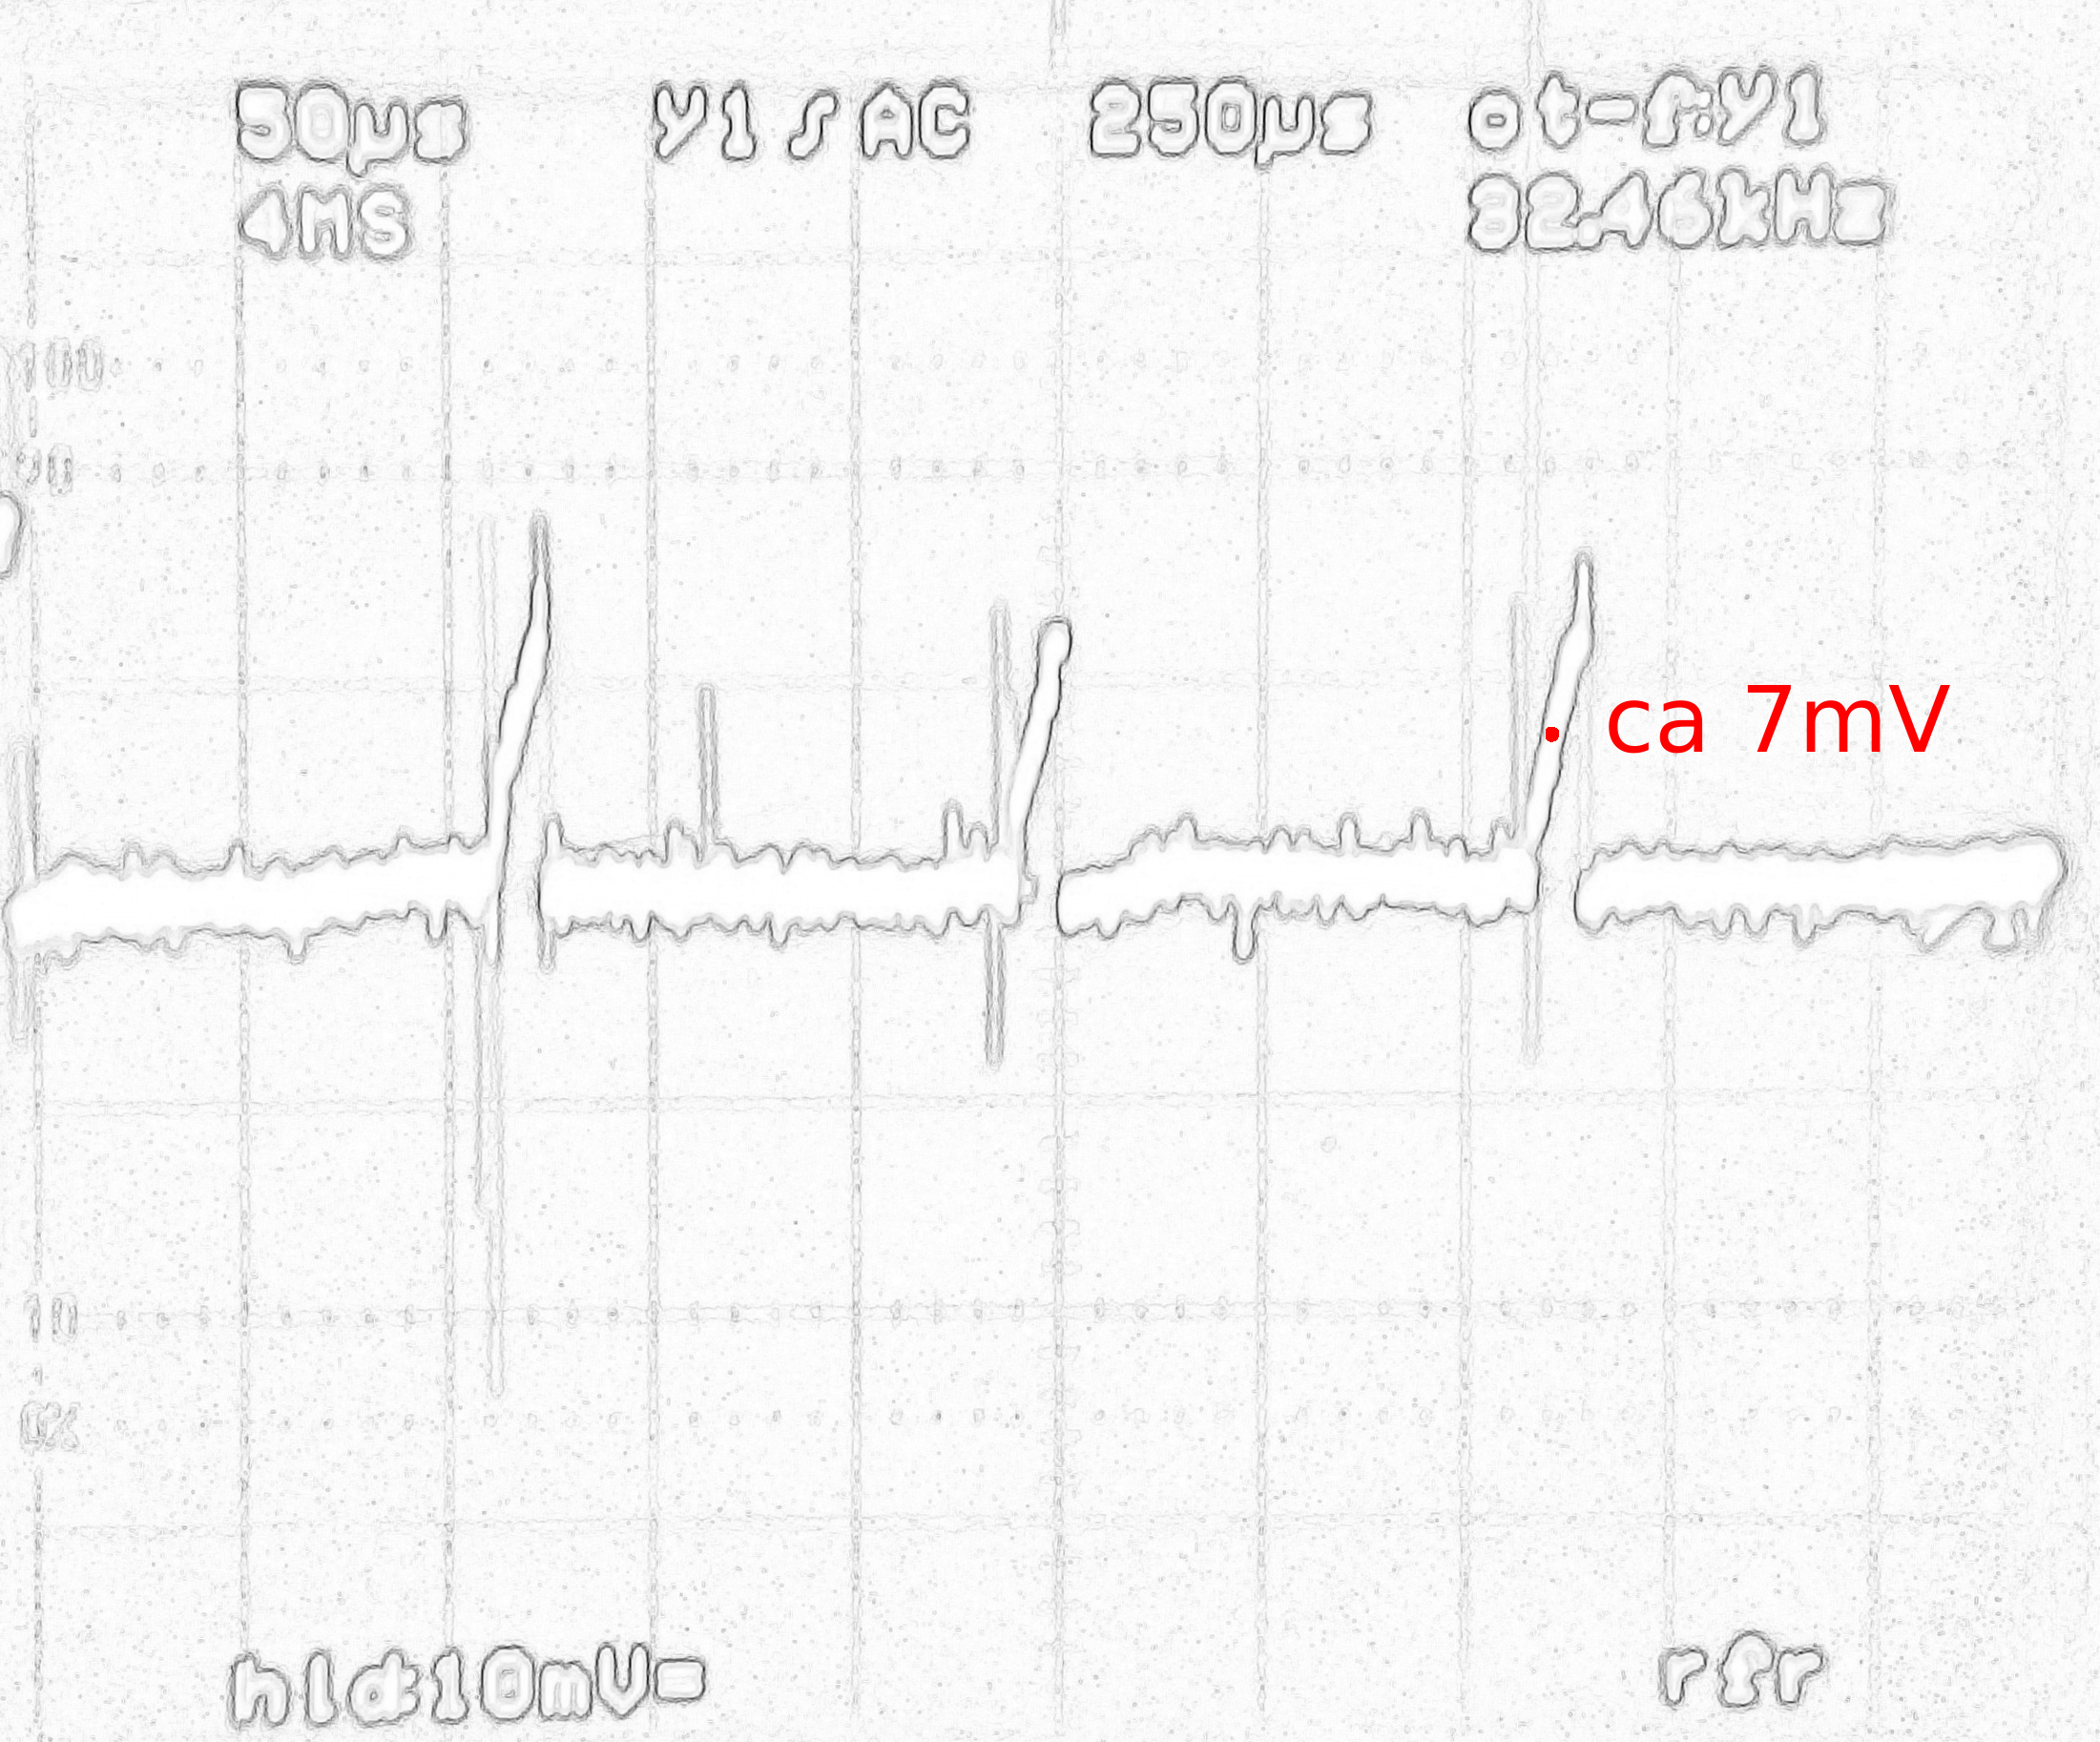
\includegraphics[width=.8\textwidth]{filter_eingang_mak.png}\\
\caption{Spannung am Shunt}%
\label{fig:filter_eingang}
\end{figure}

Die mittlere Spannung aus \cref{fig:filter_eingang} lässt sich abschätzen, indem die Spannung in der Mitte eines Impulses abgelesen und mit dem Tastverhältnis multipliziert wird.
$\SI{7}{\mV}\cdot\frac{30}{256}=\SI{0,82}{\mV} $
Mit Hilfe dieses Mittelwertes können wir grob abschätzen, ob der nachfolgende Filter seine Funktion erfolgreich erfüllt.


Als Nächstes wird die Spannung nach der Filterschaltung direkt am Operationsverstärker gemessen. Es fällt auf, dass das Signal trotz Tiefpass noch Störungen in Form des Motorstromes enthält.
Dies ist eine Auswirkung der gestörten Betriebsspannung, welche später untersucht wird.


\begin{figure}[H]
\centering
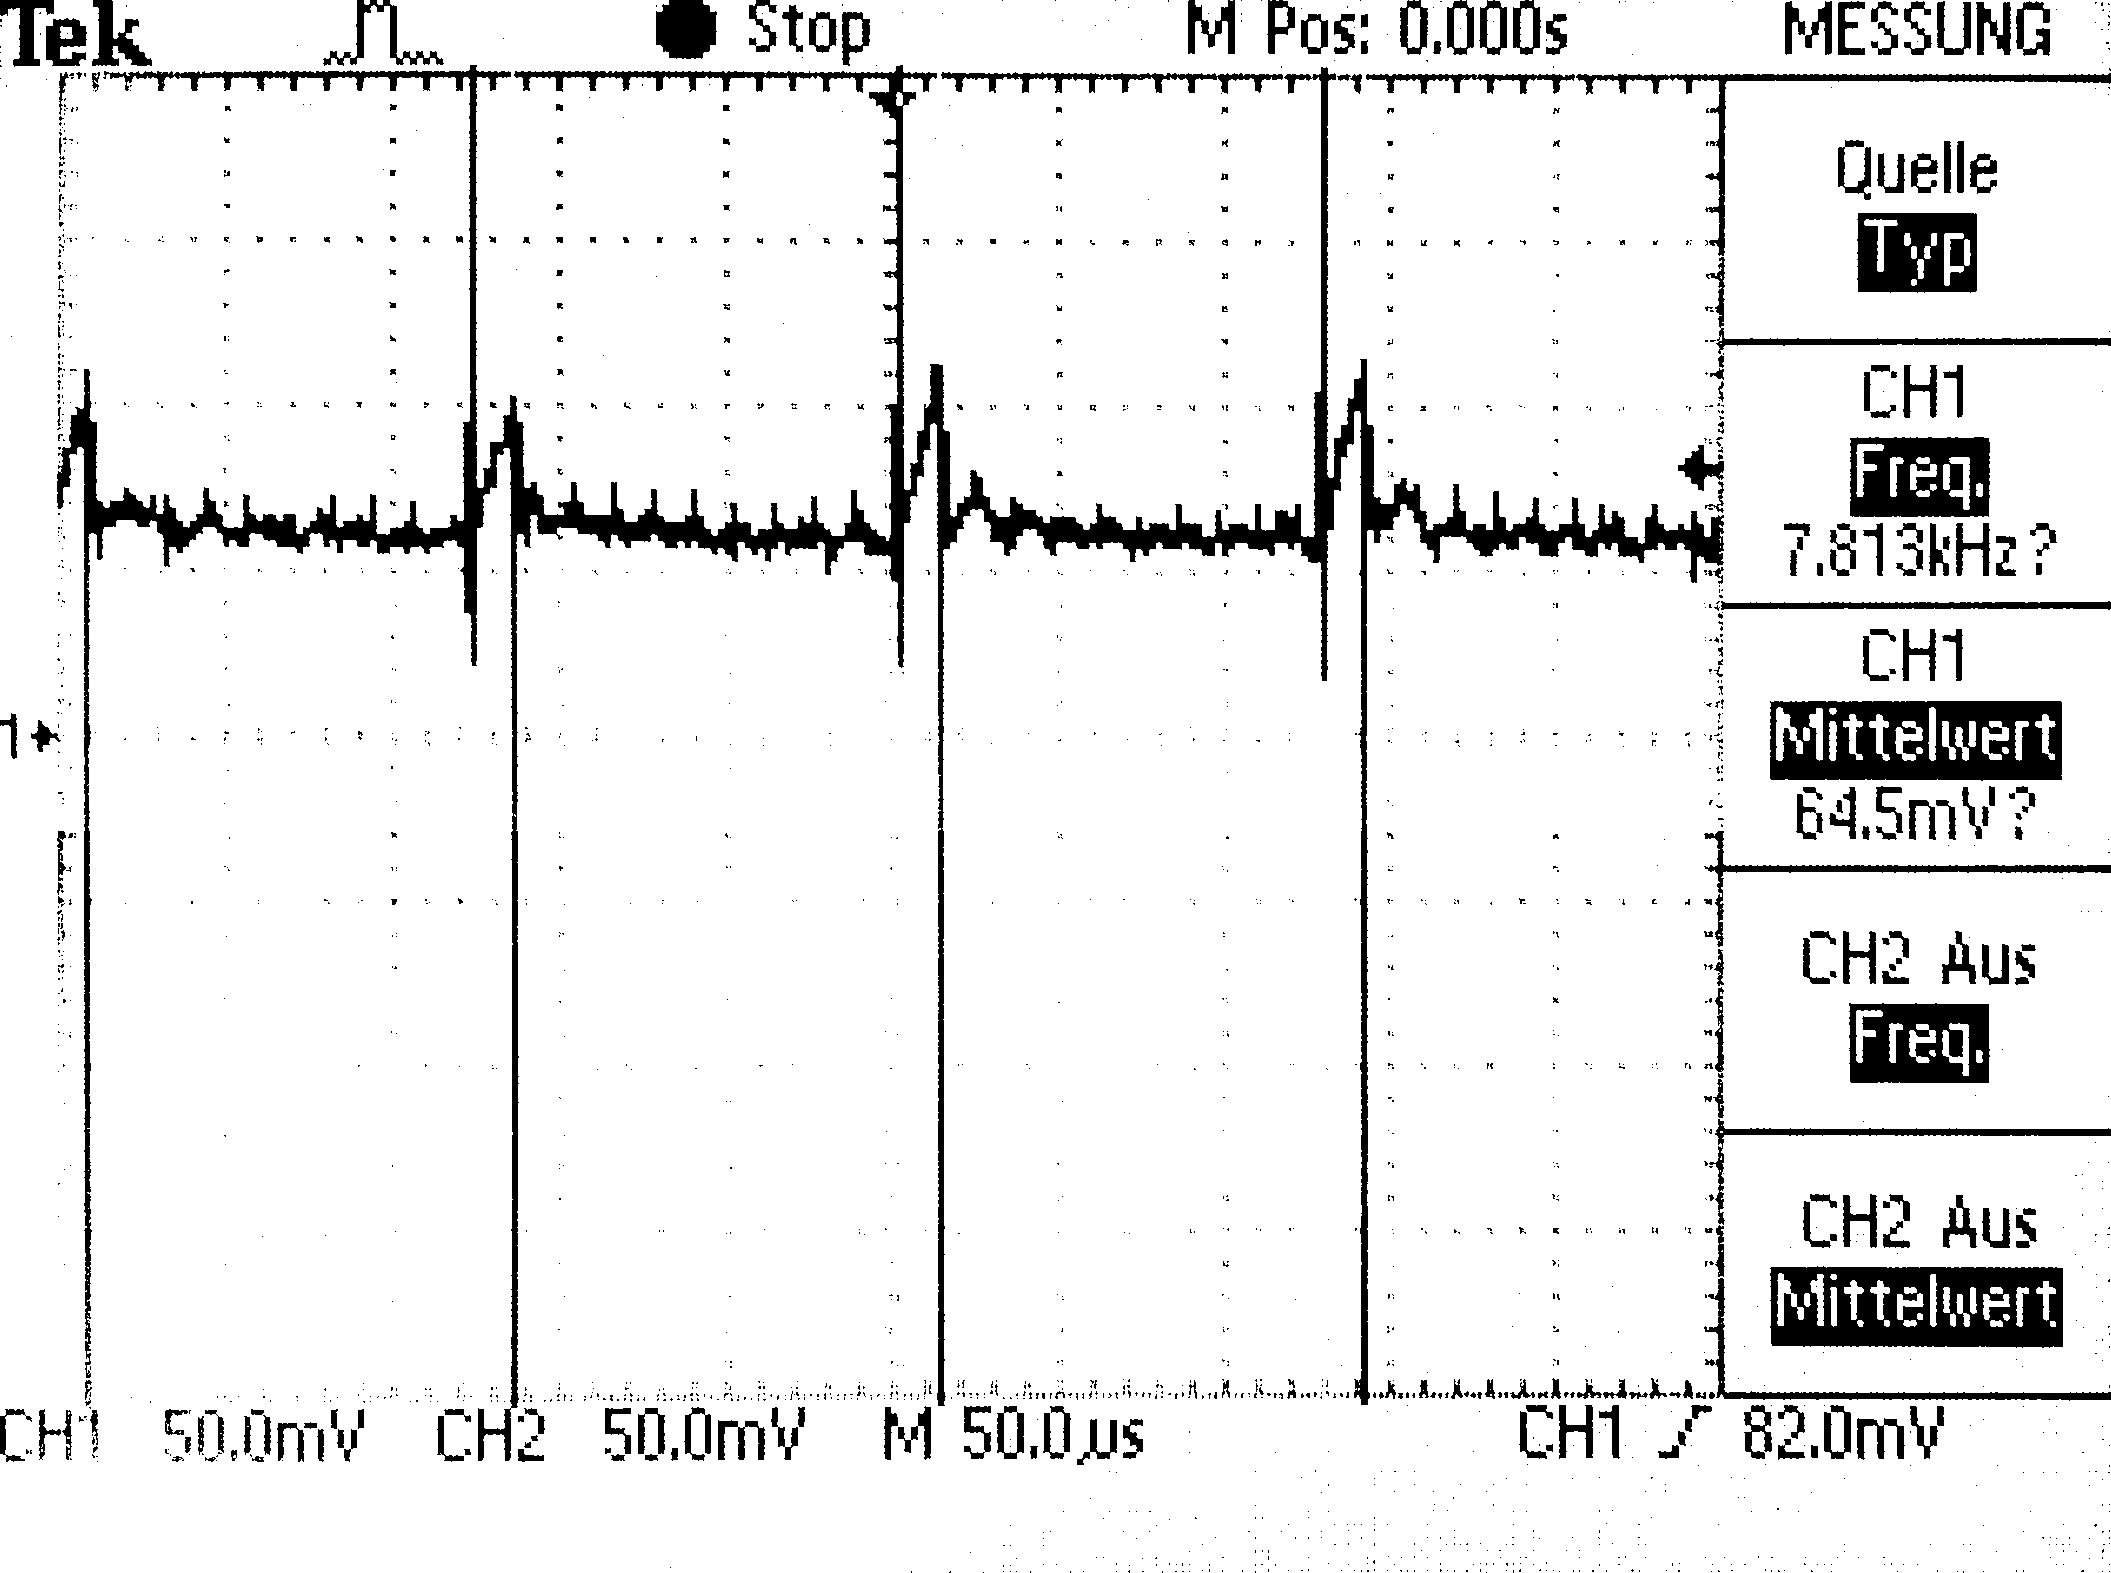
\includegraphics[width=.8\textwidth]{filter_ausgang.png}\\
\caption{Spannung nach dem Filter}%
\label{fig:filter_ausgang}
\end{figure}


Wie in \cref{fig:filter_ausgang} zu sehen wurde die Eingangsspannung erfolgreich ver\-stärkt und hat nun etwa eine Spannung von \SI{40}{\mV}. Dividiert durch den Verstärkungsfaktor 48 ergibt sich eine Spannung von 
\SI{0,83}{\mV}. Welche sehr nahe an dem vorher abgeschätzten Wert von \SI{0,82}{\mV} liegt. Der Strom lässt sich nun mit Hilfe des Ohmschen Gesetzes $U=R\cdot I$ errechnen.
\begin{align*}
I=\frac{\SI{0,83}{\mV}}{\SI{0,005}{\ohm}}=\SI{166,7}{\mA}
\end{align*}

Der vom Mikrocontroller ausgegebene Strom beträgt im Mittel \SI{156,1}{\mA}.

Zur weiteren Bewertung der Messung wurden jeweils ca. 1000 Samples an Daten zu unterschiedlichen PWM-Tastgraden aufgezeichnet.
Dabei soll untersucht werden, ob die Qualität der Messwerte mit zunehmender Geschwindigkeit stabil bleibt.
Die Ergebnisse der Messungen sind in \cref{tab:current_noload} zu sehen.
Um die Tabellen nicht zu überladen wurde der Tastgrad nur unvollständig angegeben, dieser bezieht sich immer auf Teile von 256.

\begin{table}[H]
  \centering
  \begin{tabularx}{\textwidth}{|X|r|r|}
    \hline
    Tastgrad & Erwartungswert [\si{\A}] & Standardabweichung [\si{\A}]  \\ \hline \hline
    10 & \num{0,0044} & \num{0,0212}\\ \hline
    20 & \num{0,0730} & \num{0,0214}\\ \hline
    30 & \num{0,1600} & \num{0,0215}\\ \hline
    40 & \num{0,2629} & \num{0,0214}\\ \hline
    50 & \num{0,3653} & \num{0,0185}\\ \hline
    60 & \num{0,4720} & \num{0,0231}\\ \hline

  \end{tabularx}
  \caption{Motorstrom im Leerlauf}%
  \label{tab:current_noload}
\end{table}

Die Standardabweichung der Messwerte scheint stabil zu bleiben. Da der Strom sich in diesen Messungen in einem sehr niedrigen Bereich befindet, wurden
die Messungen erneut unter Last durchgeführt, der Motor befand sich währenddessen im Kurzschlussbetrieb.

\begin{table}[H]
  \centering
  \begin{tabularx}{\textwidth}{|X|r|r|}
    \hline
    Tastgrad & Erwartungswert [\si{\A}] & Standardabweichung [\si{\A}]  \\ \hline \hline
    10 & \num{0,0454} & \num{0,0183}\\ \hline
    20 & \num{0,4635} & \num{0,0243}\\ \hline
    30 & \num{1,1694} & \num{0,0338}\\ \hline
    40 & \num{1,9822} & \num{0,0563}\\ \hline
    50 & \num{3,8737} & \num{0,0477}\\ \hline
    60 & \num{4,7023} & \num{0,0706}\\ \hline
  \end{tabularx}
  \caption{Motorstrom unter Last}%
  \label{tab:current_load}
\end{table}

Der Tabelle \ref{tab:current_load} kann leicht entnommen werden, dass die Ströme unter Last stark ansteigen. Die Standardabweichung steigt im Verhältnis zum Strom nur leicht.
Sodass die Streuung der Messung mit steigendem Strom zwar zunimmt, die relative Abweichung der Werte jedoch nicht zunimmt.


\section{Spannungsversorgung}

Während der Untersuchung der Strommessung sind Störungen im Ausgabesignal der Filterschaltung festgestellt worden. Um die Ursache der Störung zu finden, wurde die Spannungsversorgung
des Fahrzeuges untersucht.

\begin{figure}[H]
\centering
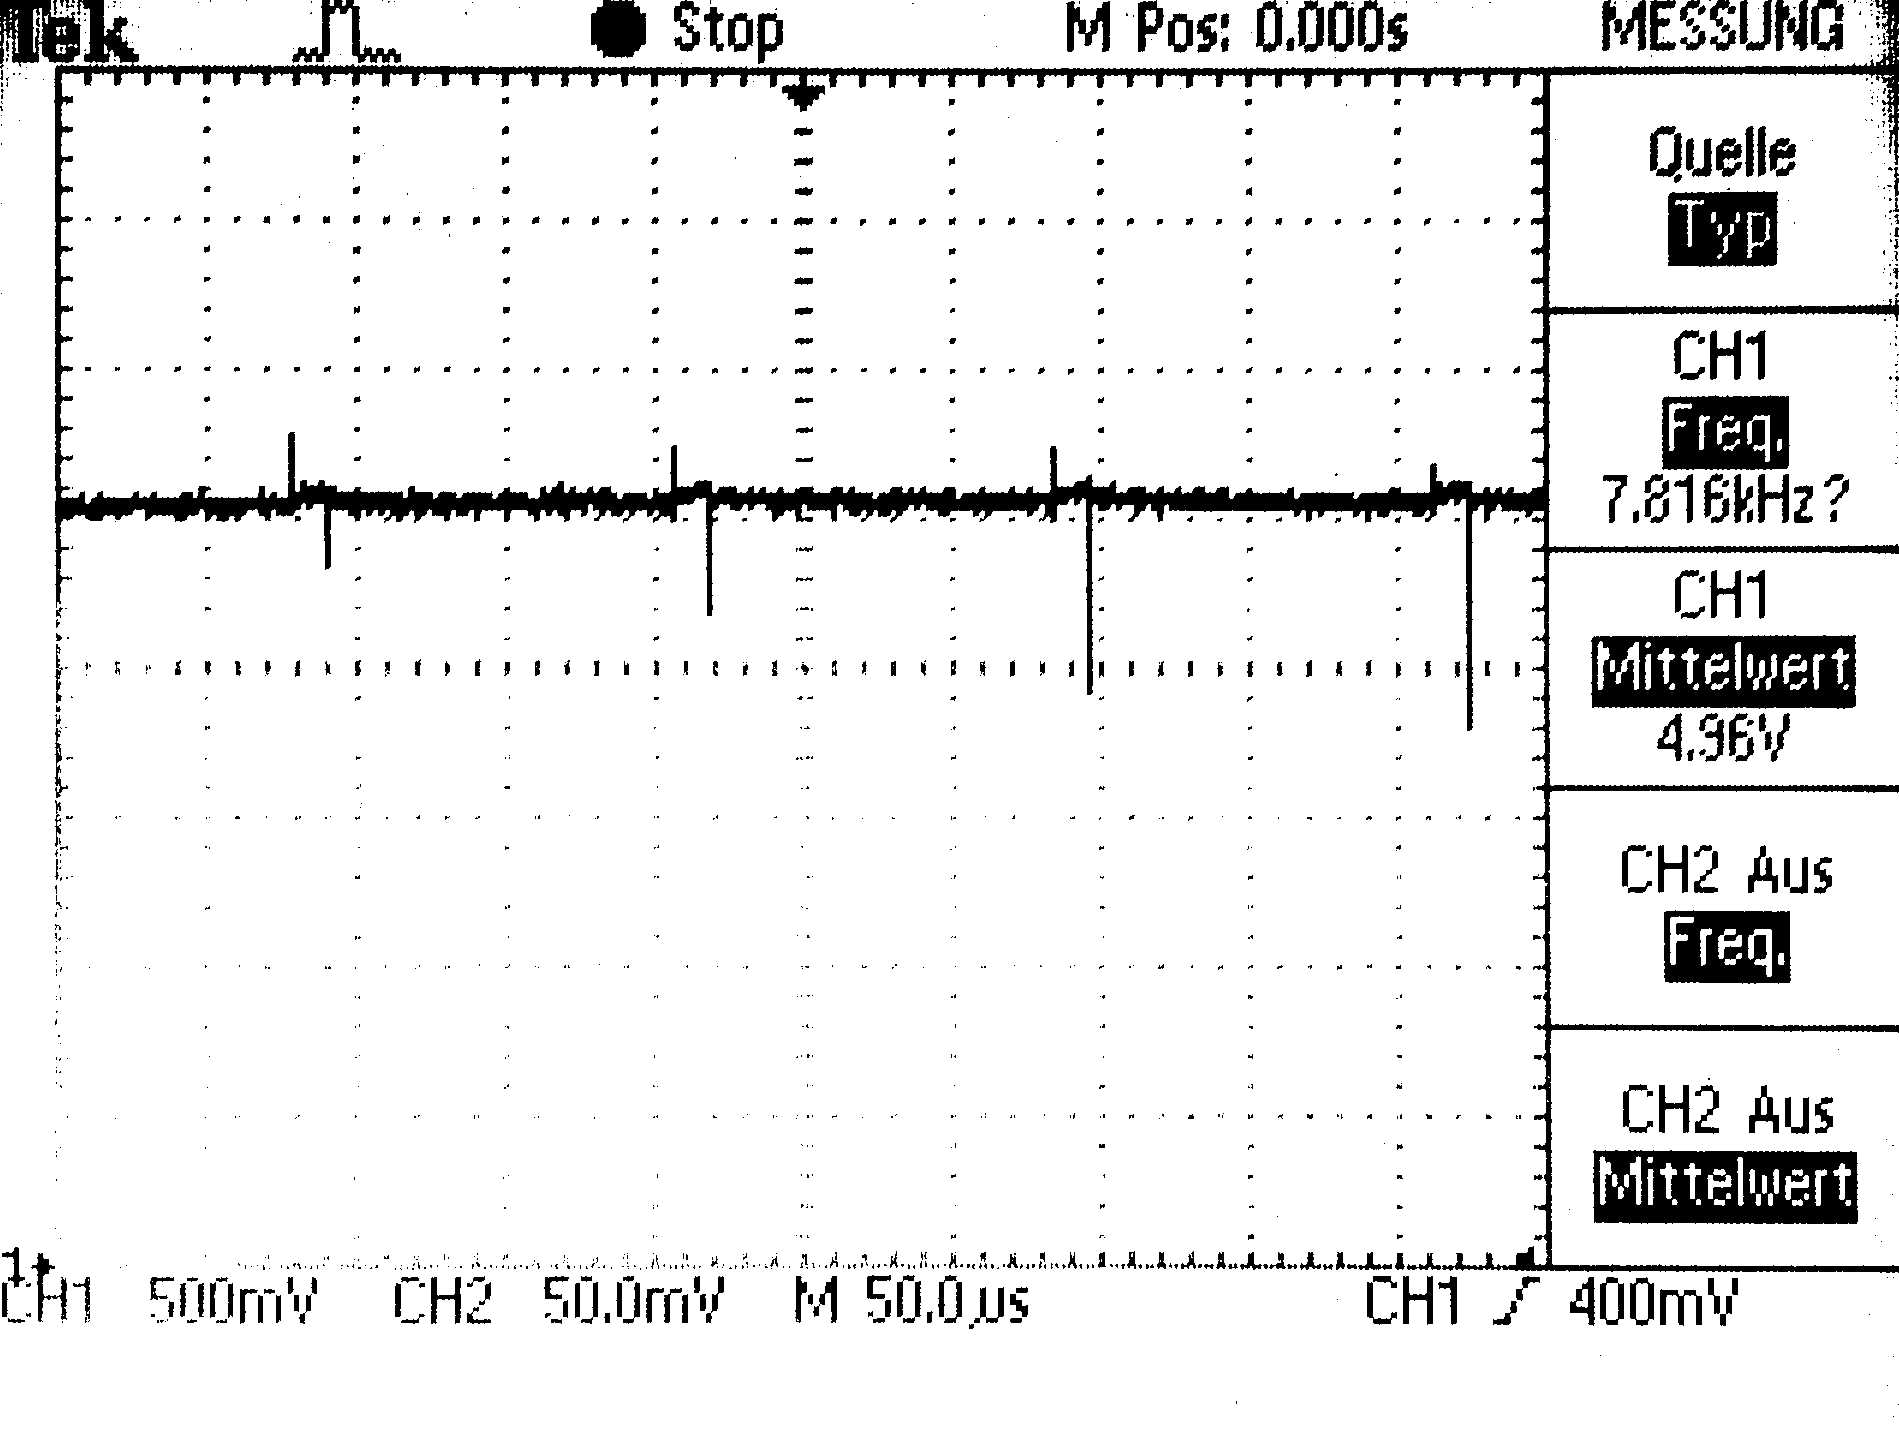
\includegraphics[width=.8\textwidth]{5V_supply.png}\\
\caption{Störungen im \SI{5}{\V} Netz}%
\label{fig:5V_Supply}
\end{figure}

Betrachtet man den Verlauf der Spannung im \SI{5}{\V}-Netz lässt sich leicht erkennen, dass das Signal von einem dem Strom sehr ähnlichen Signal überlagert wird.
Eine solche Störung kann nur von der Betriebsspannung kommen, da der Motor nicht an das \SI{5}{\V}-Netz angeschlossen ist. Scheinbar ist der \SI{5}{\V}-Schaltregler nicht in der
Lage diese Störungen vollständig auszugleichen.
Daher wird nun die Betriebsspannung untersucht, um das Ausmaß der Störungen beurteilen zu können.
Die Werte wurden in einer 1:10 Teilung gemessen, daher sind alle Spannungen mit dem Faktor 10 zu multiplizieren.

Im Akkubetrieb (\cref{fig:accu_supply}) kann gut beobachtet werden, dass die Spannung um mehr als \SI{100}{\mV} schwankt. Die Frequenz der Spannungseinbrüche entspricht in etwa
der PWM Frequenz von \SI{7812,5}{\hertz}.  Der Motor wurde währenddessen mit einem Tastgrad von 30:256 angesteuert und wurde nicht belastet.


\begin{figure}[H]
\centering
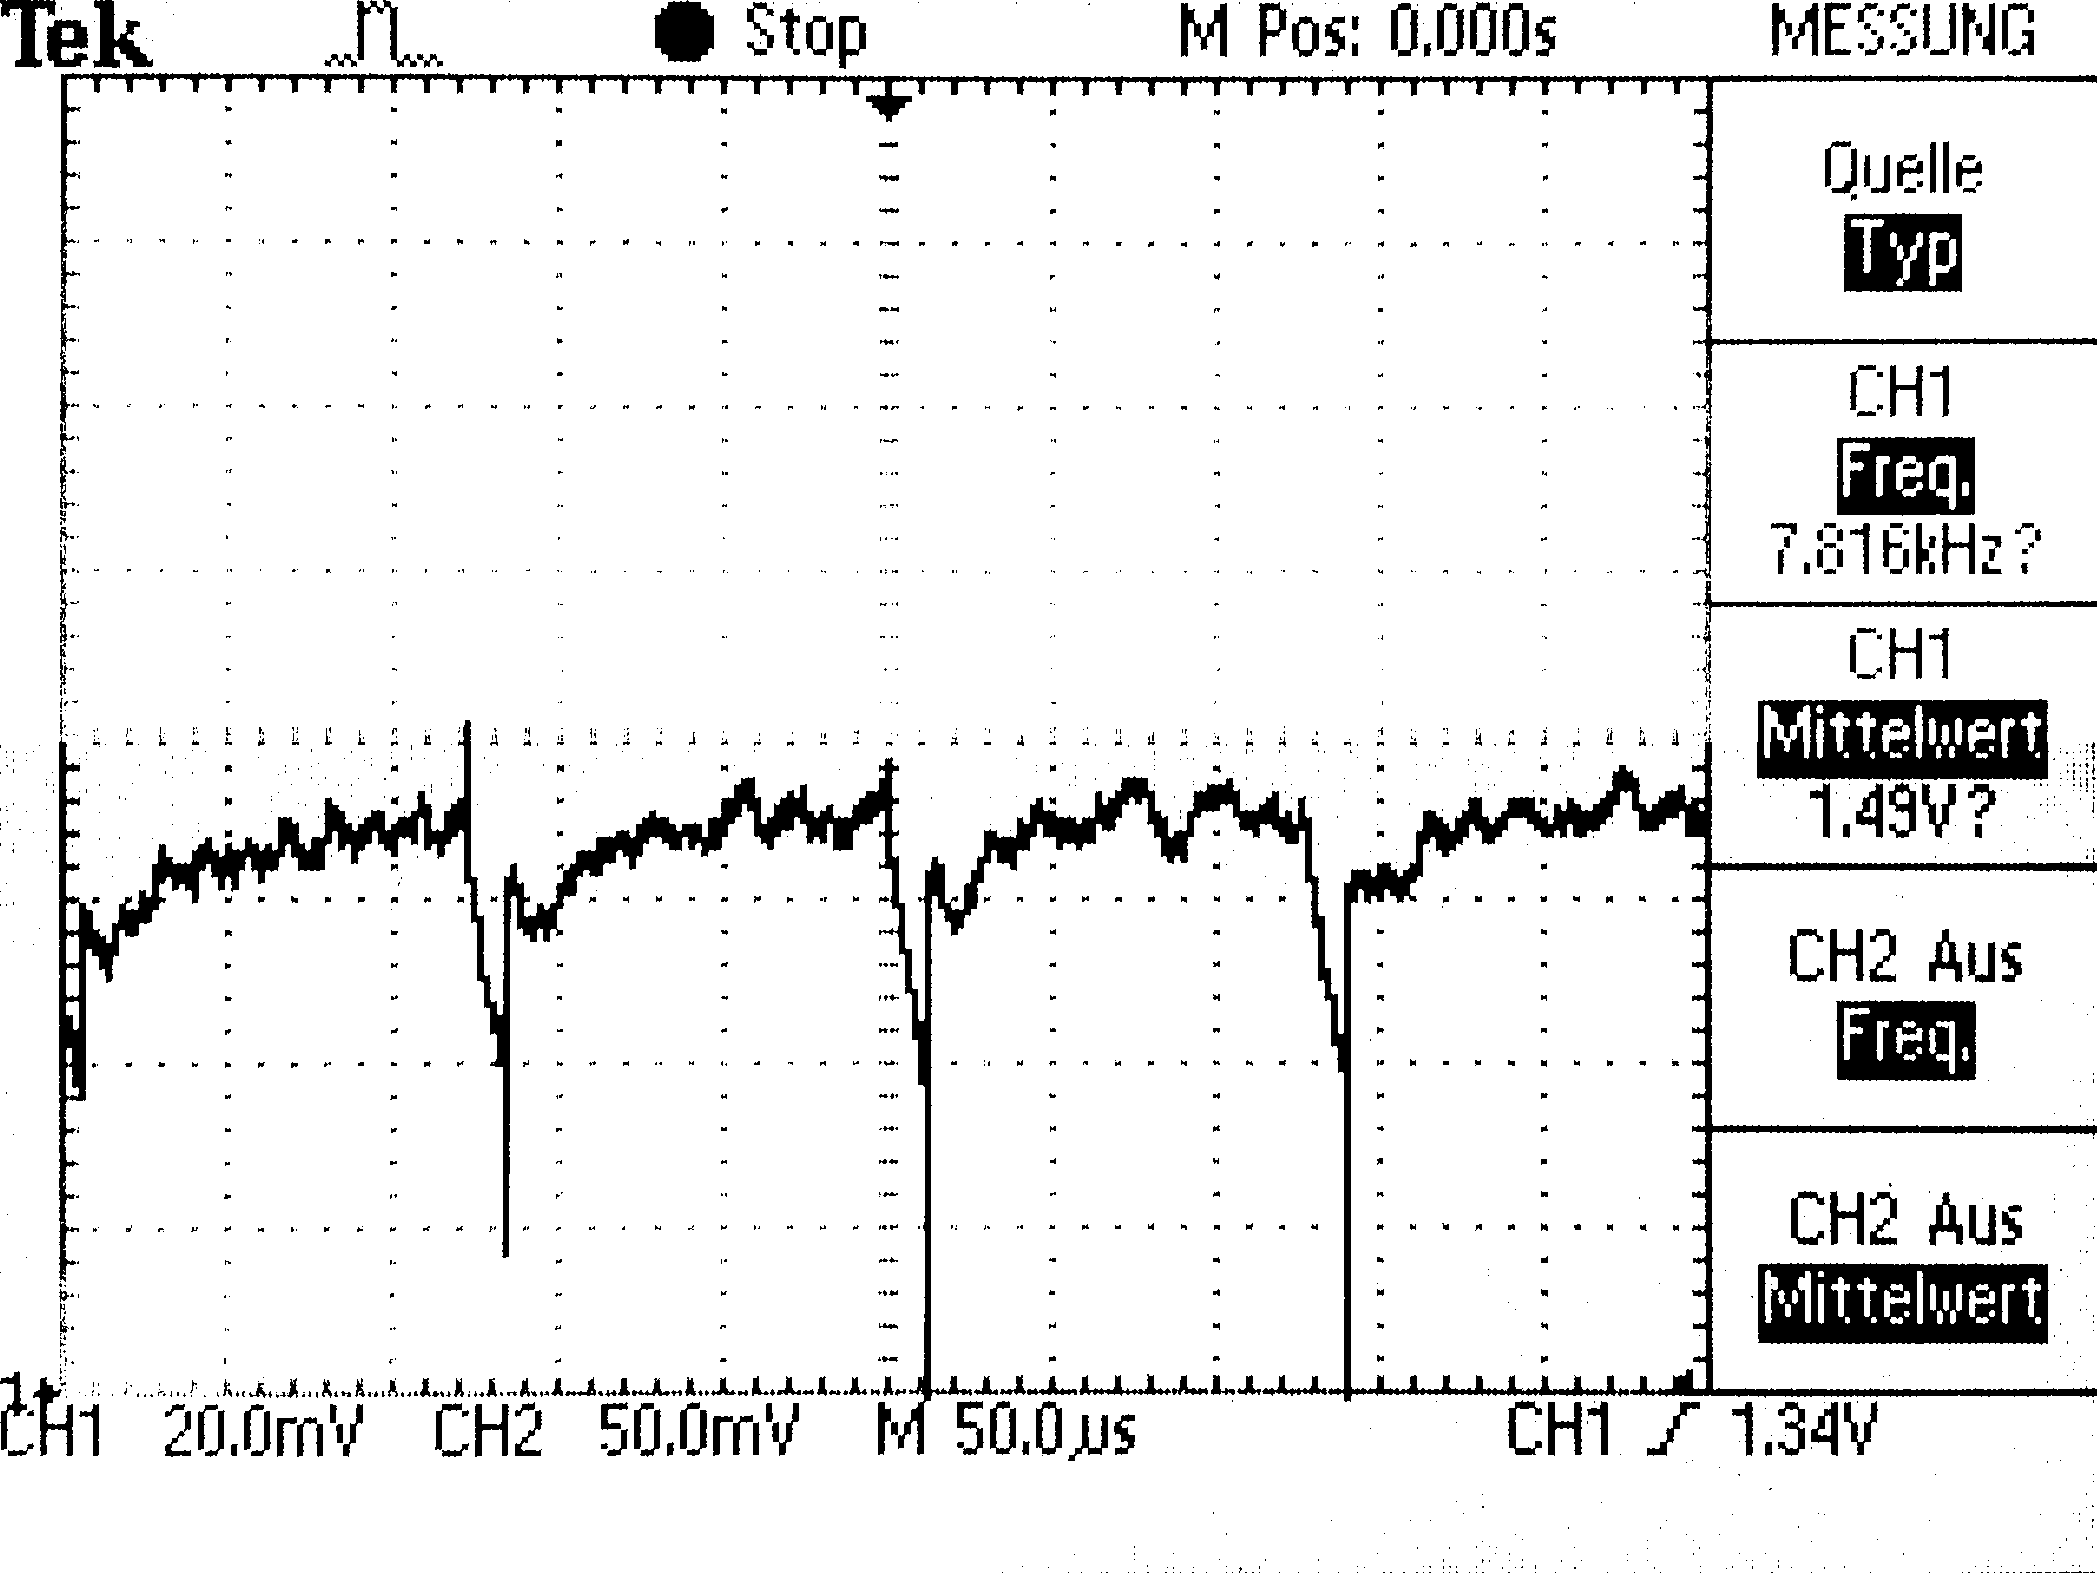
\includegraphics[width=.8\textwidth]{VCC_AKKU.png}\\
\caption{Störungen der Betriebsspannung mit Akku}%
\label{fig:accu_supply}
\end{figure}


Vergleicht man die Messungen im Akkubetrieb (\cref{fig:akku_supply}) mit den Messungen im Netzbetrieb (\cref{fig:power_supply}), kann man erkennen das das Netzteil versucht die Schwankungen auszugleichen.

\begin{figure}[H]
\centering
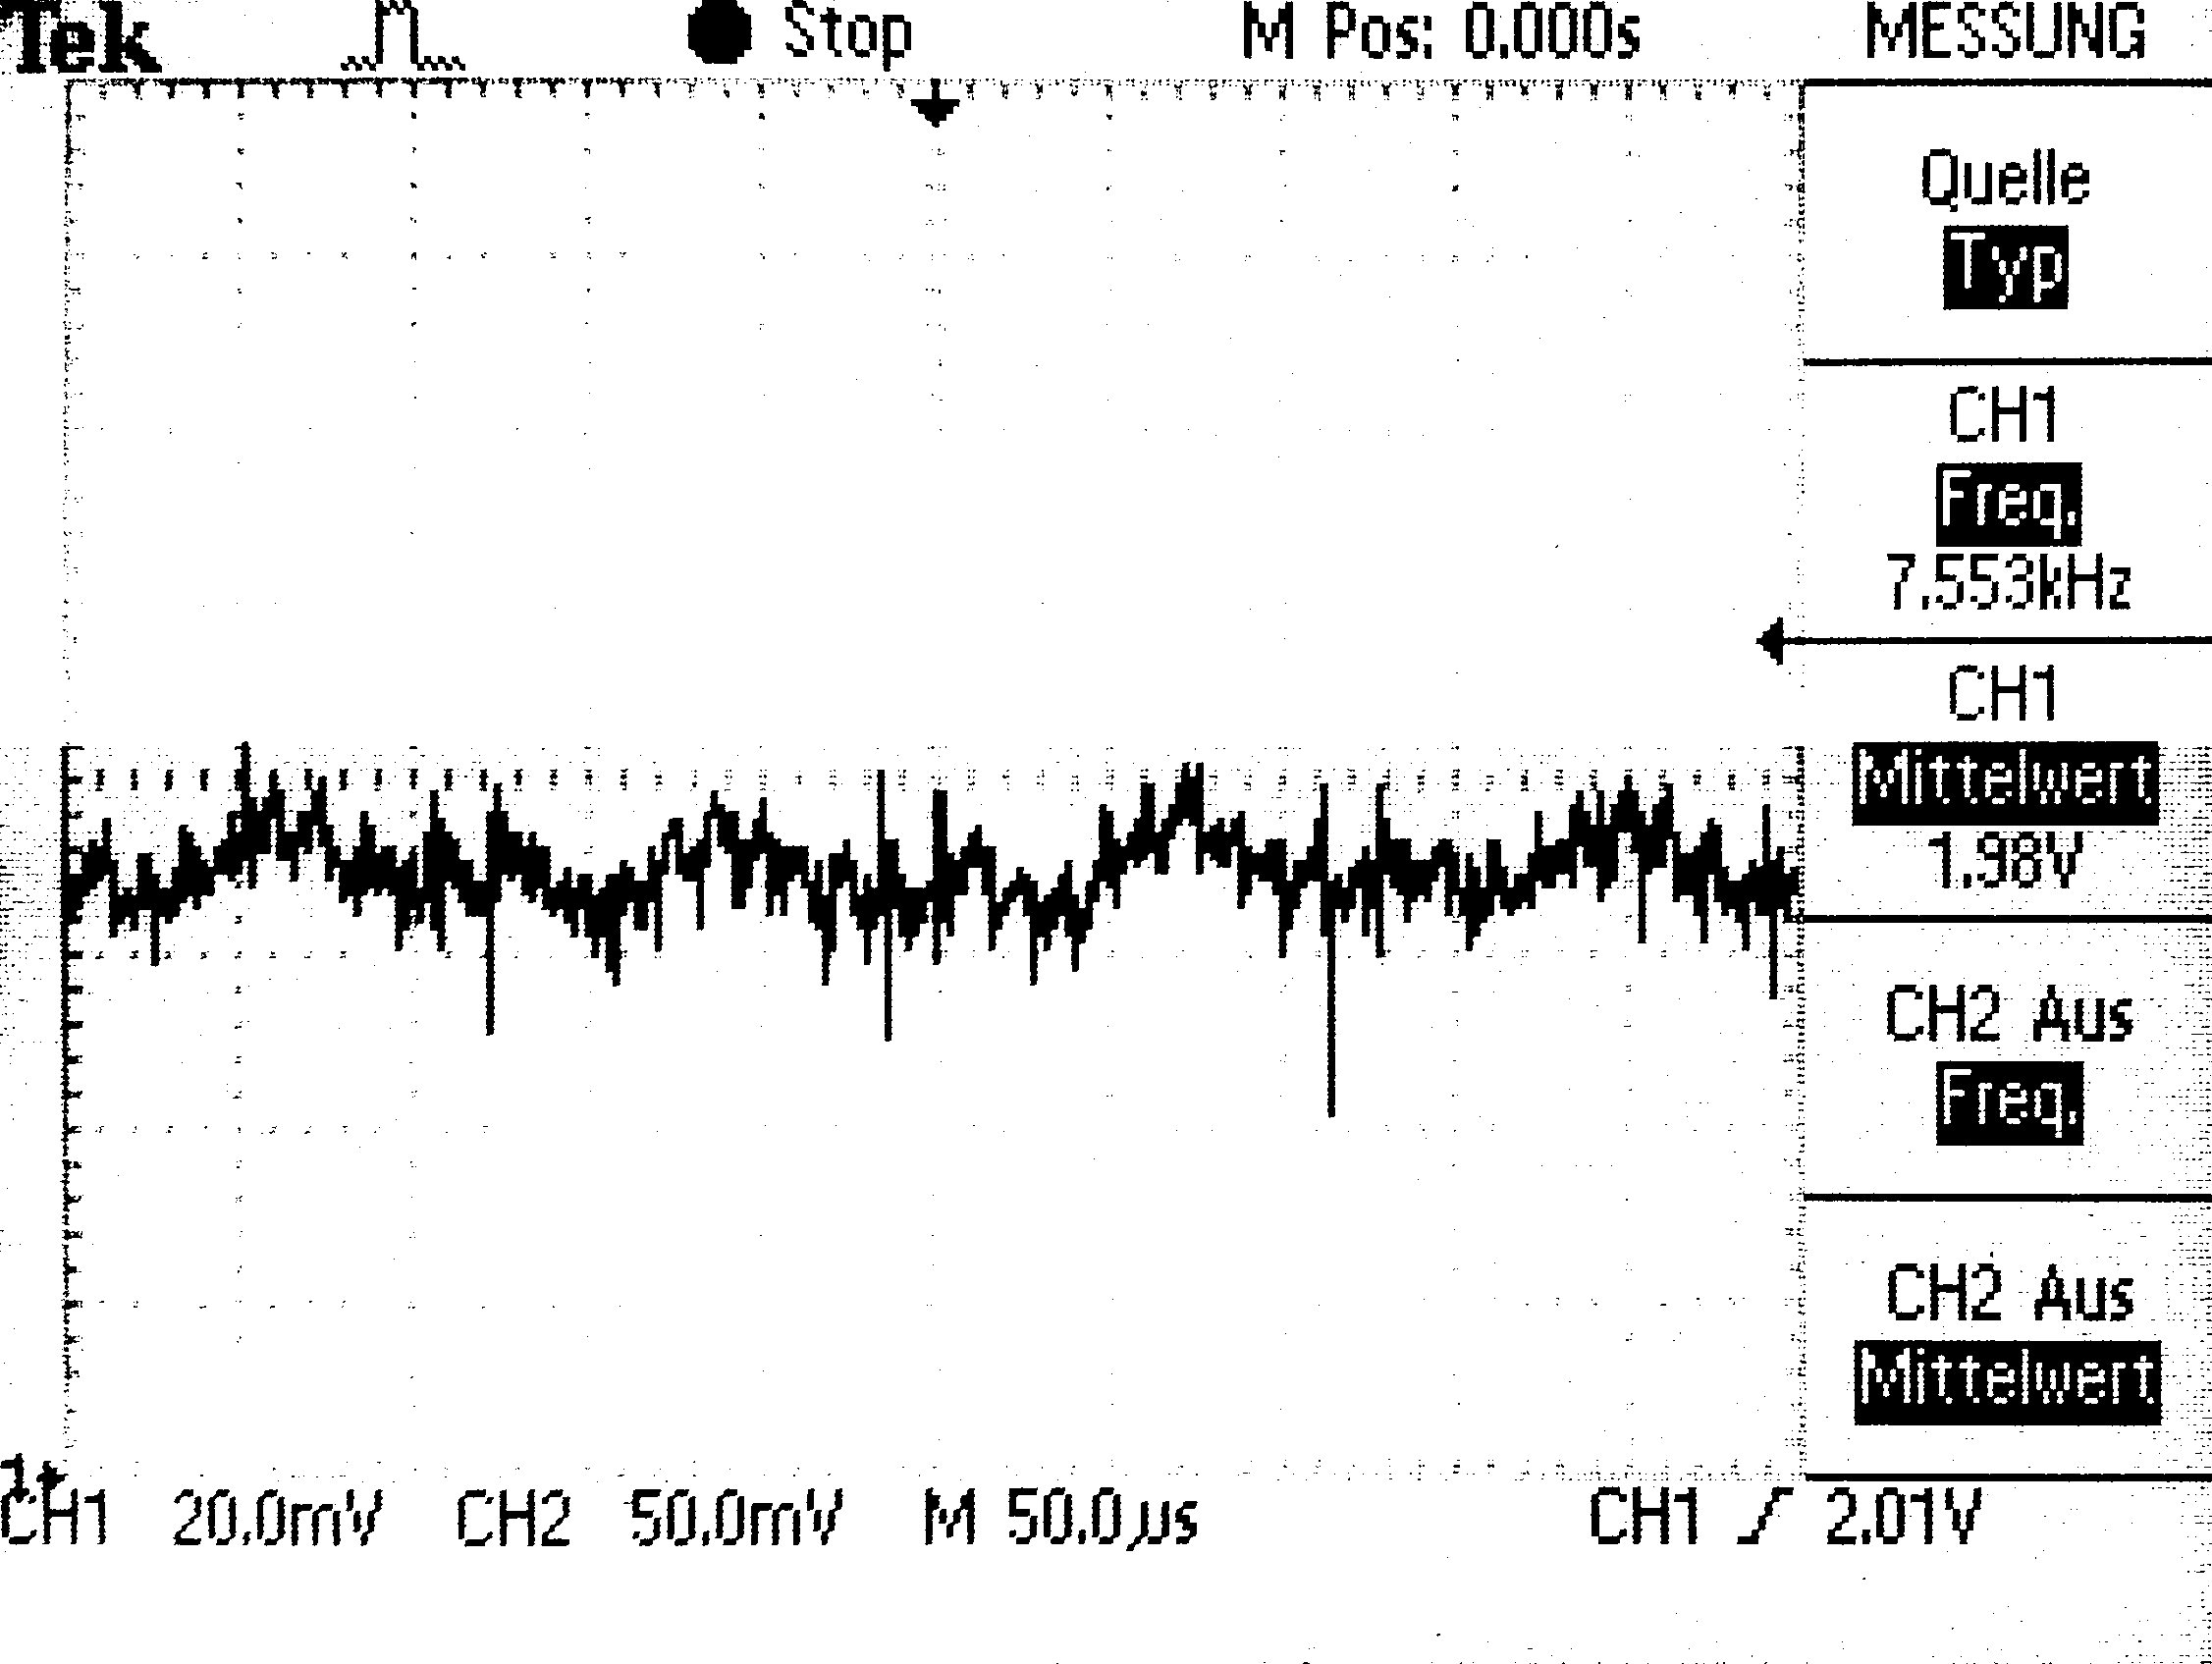
\includegraphics[width=.8\textwidth]{VCC_SUPPLY.png}\\
\caption{Störungen der Betriebsspannung mit Netzteil}%
\label{fig:power_supply}
\end{figure}

Unter Last bei einem Tastgrad von 50:256 beträgt die Amplitude der Schwankungen im Akkubetrieb über \SI{3}{V}. Die Messung wurde ohne 1:10 Teilung durchgeführt.
Erstaunlicherweise war trotz der starken Schwankungen noch ein stabiler Betrieb des Fahrzeuges möglich. Dies wurde jedoch nur ca. 30 Sekunden getestet, da
die hohe Belastung zu einer starken Wärmeentwicklung des Motors führte.

\begin{figure}[H]
\centering
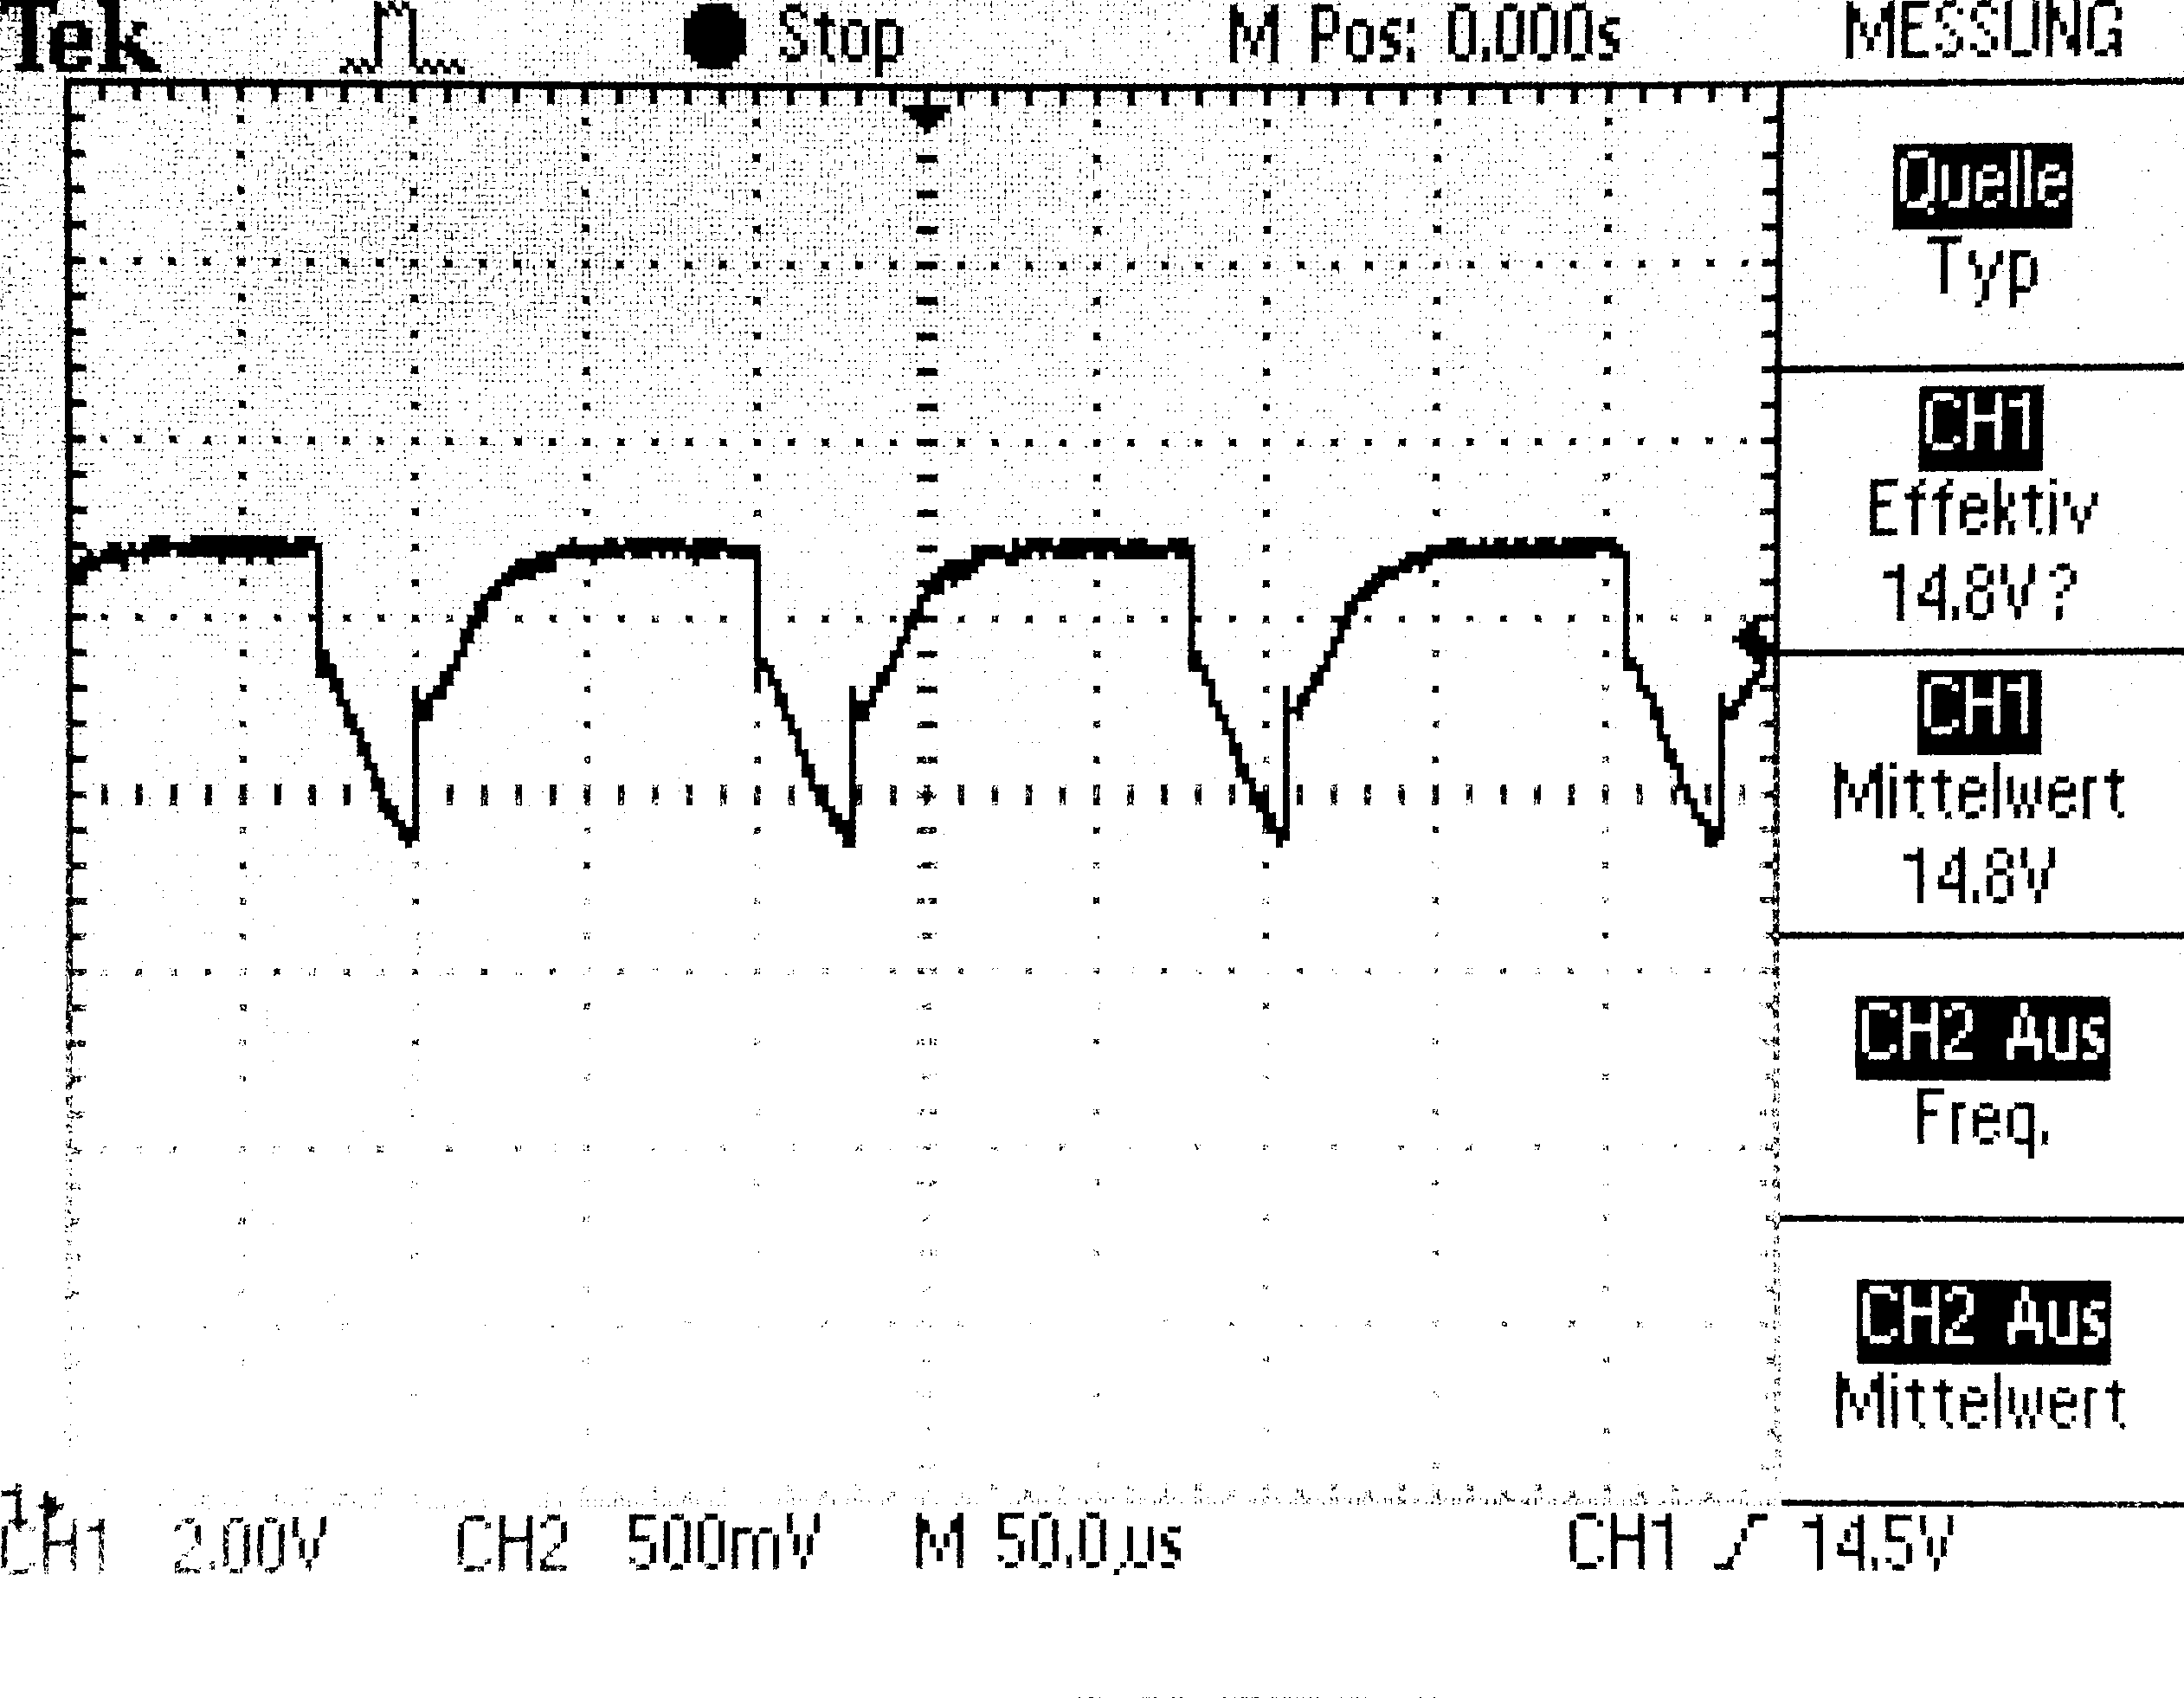
\includegraphics[width=.8\textwidth]{VCC_AKKU_LAST.png}\\
\caption{Störungen der Betriebsspannung mit Akku unter Last}%
\label{fig:akku_supply}
\end{figure}

Betrachtet man das \SI{5}{\V}-Netz unter diesen Bedingungen (\cref{fig:5V_last}) zeigt sich die beeindruckende Leistung des \SI{5}{\V} Schaltreglers.
Das \SI{5}{\V}-Netz scheint trotz der immensen Störung im Mittel noch stabil. Jedoch hat sich die Amplitude der Störungen
stark vergrößert.

\begin{figure}[H]
\centering
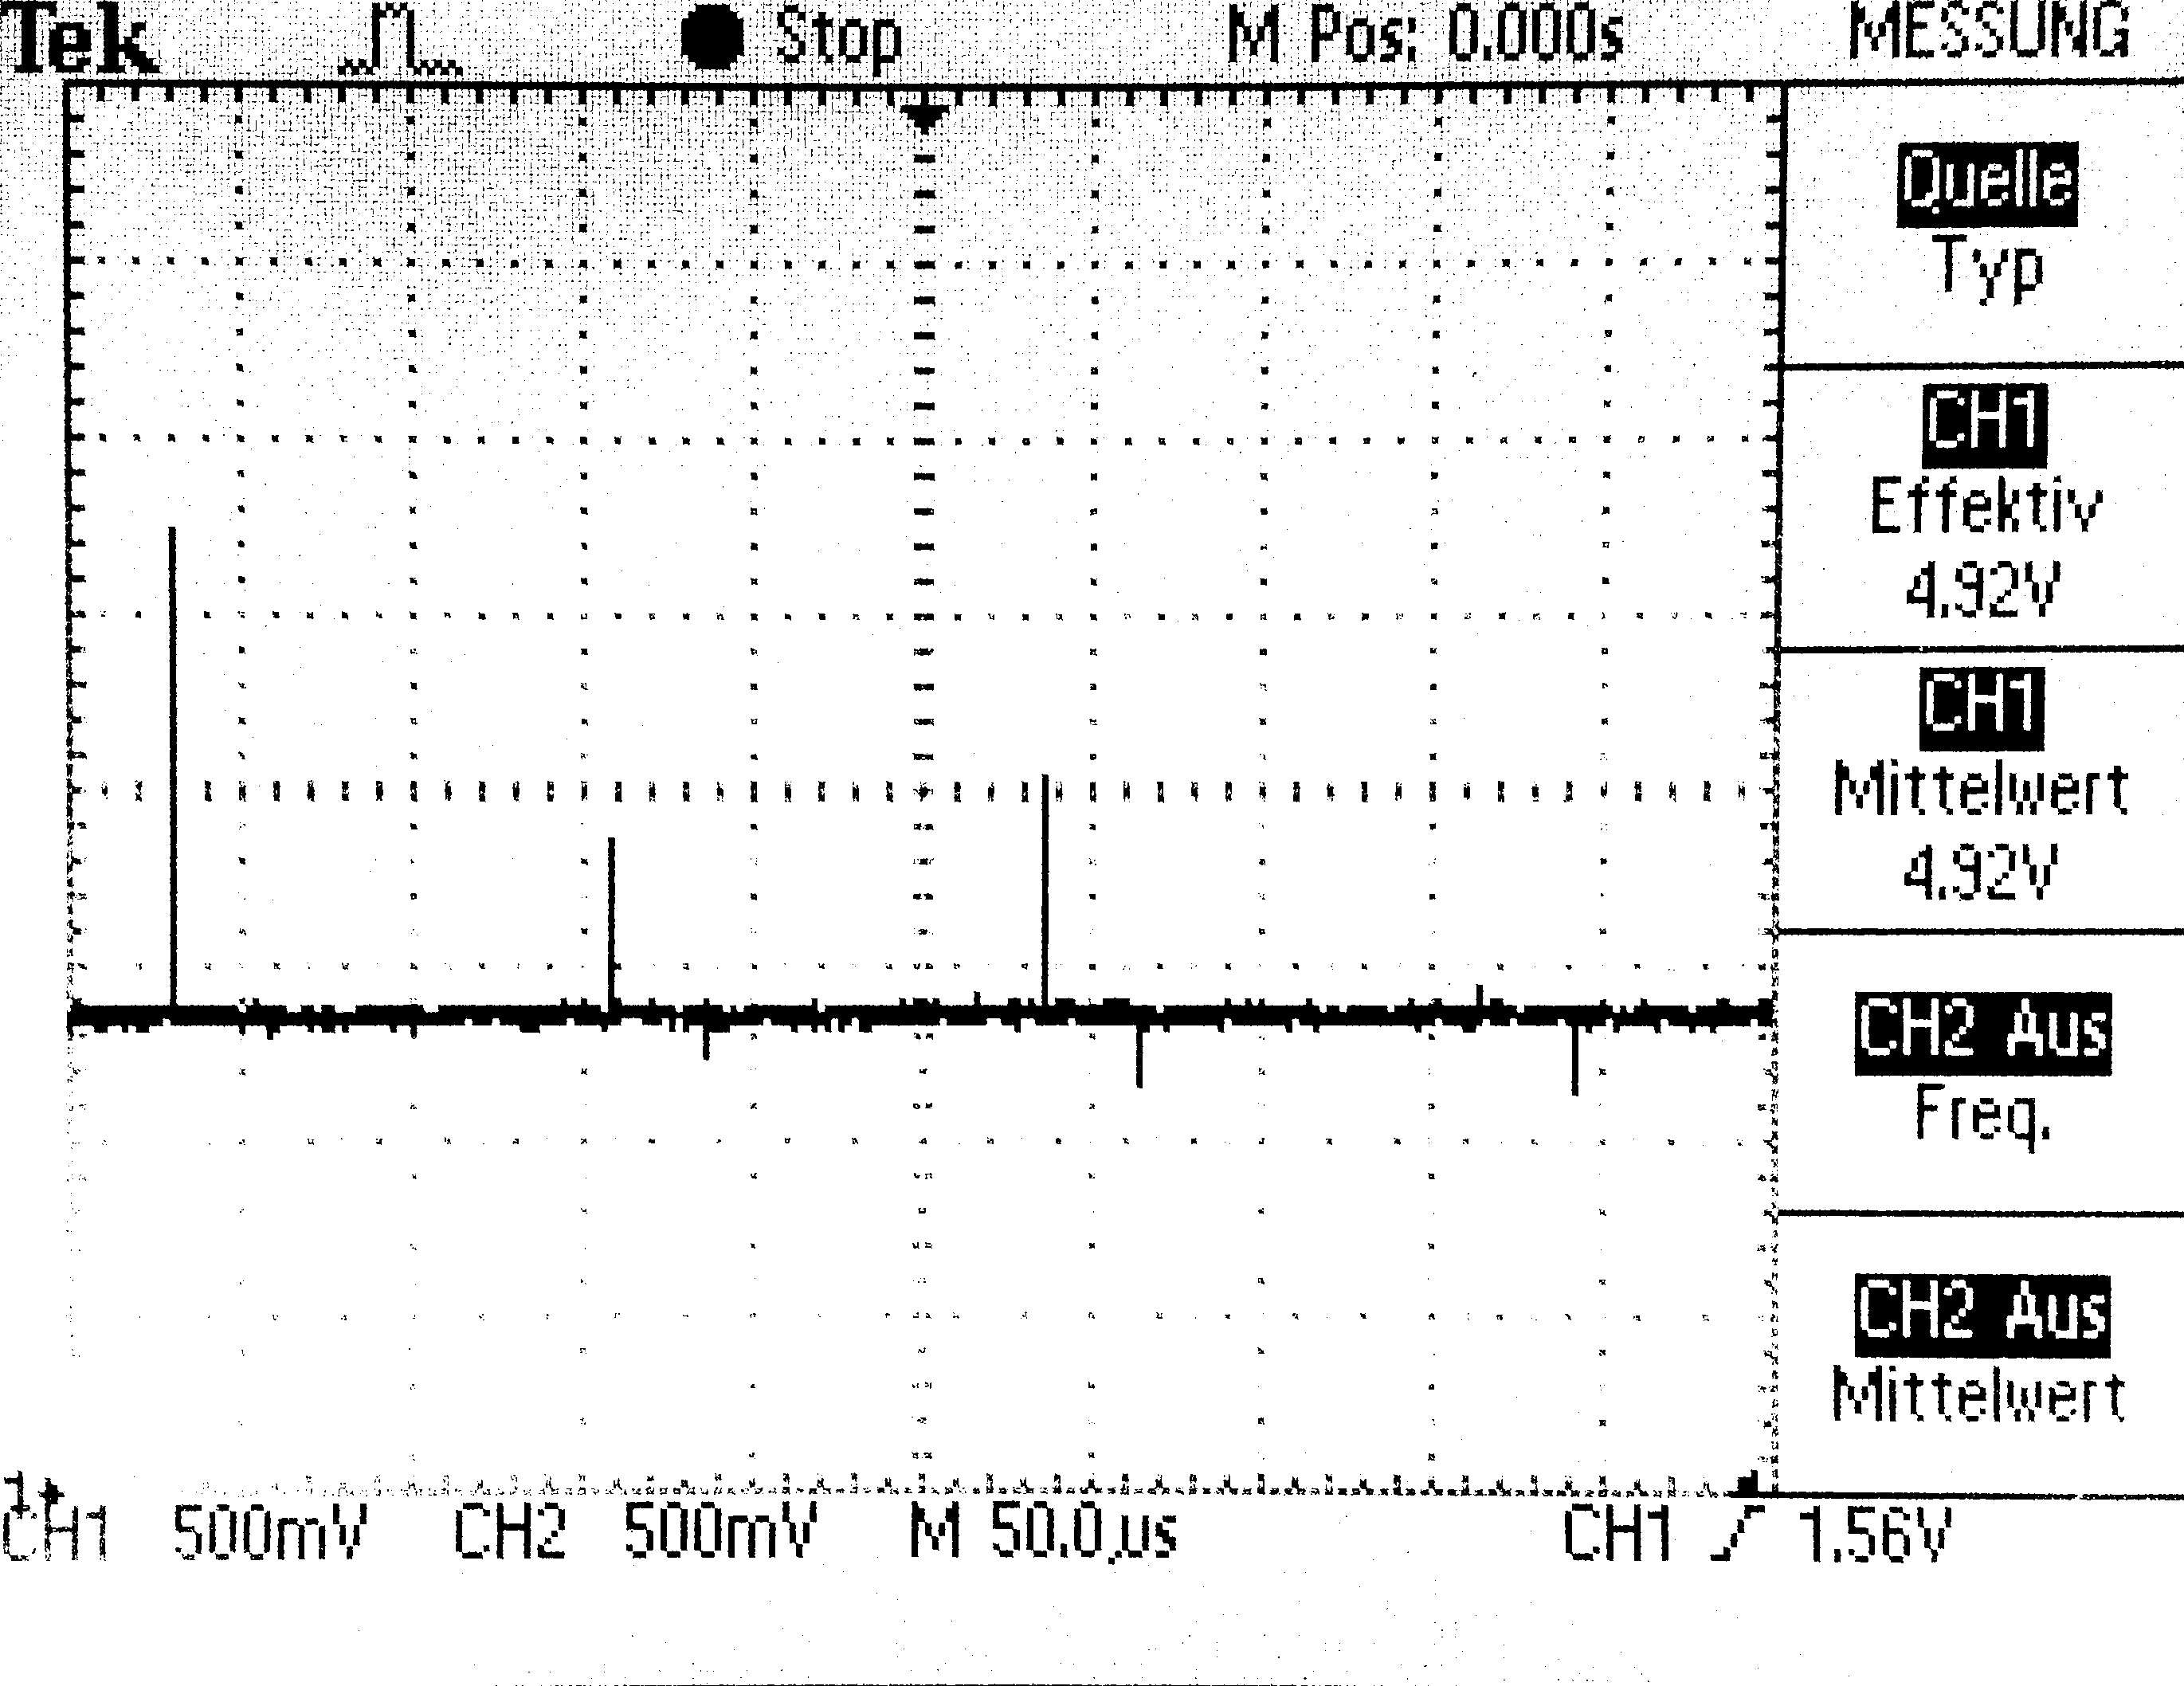
\includegraphics[width=.8\textwidth]{5V_LAST.png}\\
\caption{Störungen des \SI{5}{\V} Netzes unter Last}%
\label{fig:5V_last}
\end{figure}


Da das \SI{5}{\V}-Netz während der Motor belastet ist von Störungen überlagert ist, werden in den nächsten Abschnitten die Sensorwerte in Ab\-hän\-gig\-keit von der Motorlast untersucht.

\section{Inertialsensor}

Da die Auswertung der Inertialsensorik ist nicht Teil diese Arbeit. Um jedoch die Abhängigkeit der Inertialsensorik von der Motorlast
zu untersuchen, wurden einige Messwerte aufgenommen.

Die Messwerte wurden unter Last bei dem angegebenen Tastgrad aufgenommen. Um die Anzahl der Messwerte gering zu halten wurde legendlich die x-Achse der Sensoren untersucht.

\begin{table}[H]
  \centering
  \begin{tabularx}{\textwidth}{|X|r|r|}
    \hline
     Tastgrad & Erwartungswert [\si{\metre\per\second\squared}] & Standardabweichung [\si{\metre\per\second\squared}]  \\ \hline \hline
     20 & \num{-0,02034}  & \num{0,00078} \\ \hline
     30 & \num{-0,02047}  & \num{0,00225} \\ \hline
     40 & \num{-0,02035}  & \num{0,00097} \\ \hline
     50 & \num{-0,02034}  & \num{0,00074} \\ \hline
     60 & \num{-0,02028}  & \num{0,00189} \\ \hline
  \end{tabularx}
  \caption{Accelerometer}%
  \label{tab:acc}
\end{table}

\begin{table}[H]
  \centering
  \begin{tabularx}{\textwidth}{|X|r|r|}
    \hline
     Tastgrad & Erwartungswert [\si{\radian\per\second}] & Standardabweichung [\si{\radian\per\second}]  \\ \hline \hline
     20 & \num{0,72961} & \num{0,27632}\\ \hline
     30 & \num{0,77174} & \num{0,30825}\\ \hline
     40 & \num{0,78556} & \num{0,27121}\\ \hline
     50 & \num{0,77792} & \num{0,27066}\\ \hline
     60 & \num{0,87919} & \num{0,23369}\\ \hline
  \end{tabularx}
  \caption{Gyroskop}%
  \label{tab:gyro}
\end{table}


Sowohl beim Accelerometer als auch beim Gyroskop lässt sich anhand der Daten keine Abhängigkeit erkennen.

\begin{table}[H]
  \centering
  \begin{tabularx}{\textwidth}{|X|r|r|}
    \hline
     Tastgrad & Erwartungswert [\si{\tesla}] & Standardabweichung [\si{\tesla}]  \\ \hline \hline
     20 & \num{0,06974} & \num{0,00436}\\ \hline
     30 & \num{0,07602} & \num{0,00715}\\ \hline
     40 & \num{0,07336} & \num{0,01154}\\ \hline
     50 & \num{0,06504} & \num{0,01366}\\ \hline
     60 & \num{0,06564} & \num{0,01894}\\ \hline
  \end{tabularx}
  \caption{Magnetometer}%
  \label{tab:mag}
\end{table}

Beim Magnetometer lässt sich jedoch erkennen, dass die Streuung der Daten mit zunehmender Motorlast ebenfalls zunimmt. Da der Motor jedoch ein Magnetfeld
erzeugt, welches mit zunehmender Belastung zunimmt, war ein Einfluss auf die Messwerte zu erwarten. Diese Störungen sollten bei der Verwendung
des Magnetometers beachtet werden.


Weiter Störungen beim Magnetometer entstehen, wenn der Servomotor belastet wird (\cref{plott:ripple_mag}). Durch die Art und Weise wie der Servomotor arbeitet, treten starke Schwankungen im Stromverbrauch des Servomotors auf.
Bei der Untersuchung des \SI{5}{\V}-Netzes konnten allerdings keine Störungen in der Spannungsversorgung festgestellt werden.


  
\begin{figure}[H]
\centering
\begin{gnuplot}[terminal=pdf, scale=0.94]
  set nokey
  set xlabel 'Zeit in [s]'
  set ylabel 'Flussdichte in [T]'
  set datafile separator ','
  plot 'MessData/Imu-servo/mit_stoerung.csv' with line
\end{gnuplot}
\caption{Störungen des Magnetometers}
\label{plott:ripple_mag}
\end{figure}

Nach ausführlicher Untersuchung konnte der Fehler jedoch im Platinenlayout ausgemacht werden.

\begin{figure}[H]
\centering
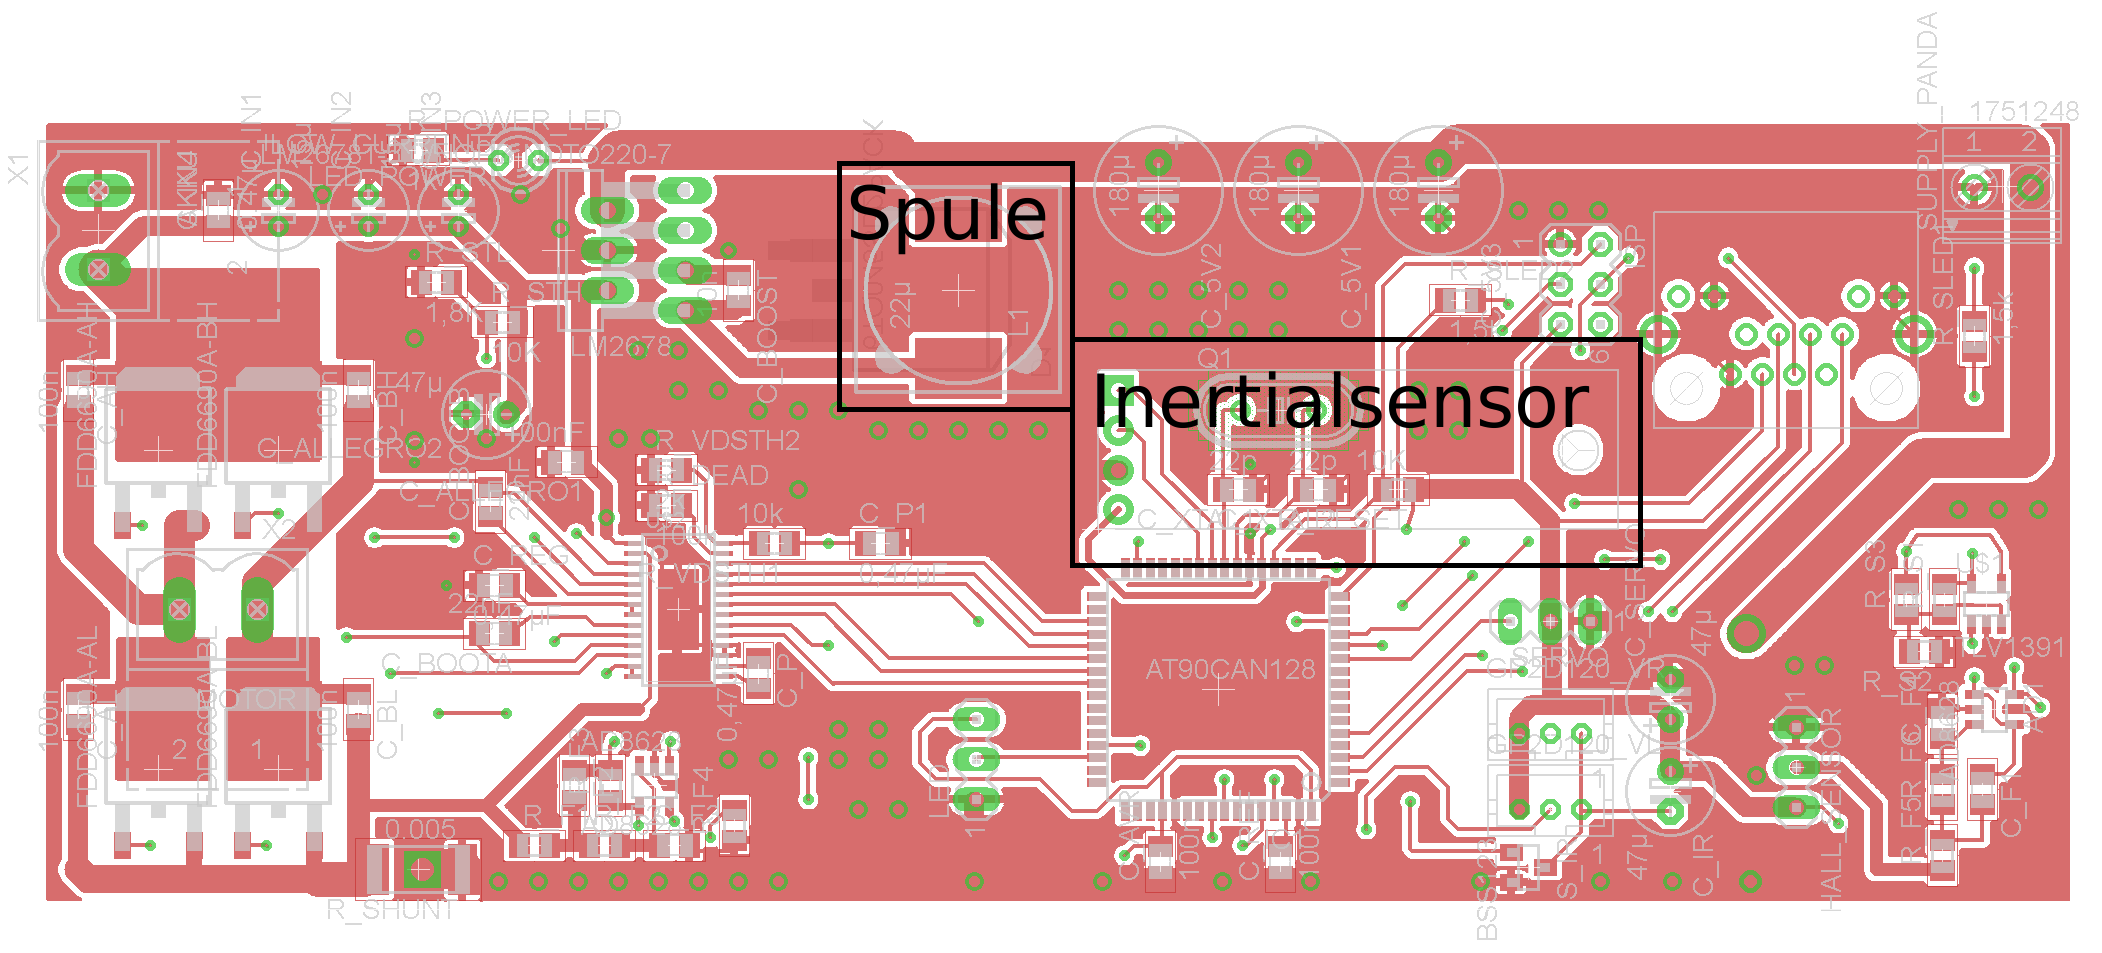
\includegraphics[width=.8\textwidth]{platine_imu.png}\\
\caption{Platinenlayout mit IMU und Spule}%
\label{fig:plat_imu}
\end{figure}

Der Inertialsensor wurde bei der Entwicklung des Layouts zu nahe an die Filterspule des Schaltreglers gelegt. Da das Magnetfeld einer Spule proportional zum durchfließenden Strom ist, treten die Störungen
besonders bei starken Lastwechseln im \SI{5}{\V}-Netz auf. Die konstante Belastung belegt das Magnetometer nur mit einem Offset.

Durch die Verschiebung des Inertialsensors, mit Hilfe einer Lochrasterplatine, konnten die Störungen jedoch stark verringert werden (siehe \cref{plott:ripple_mag_new}).

\begin{figure}[H]
\centering
\begin{gnuplot}[terminal=pdf, scale=0.94]
  set nokey 
  set xlabel 'Zeit in [s]'
  set ylabel 'Flussdichte in [T]'
  set datafile separator ','
  plot 'MessData/Imu-servo/ohne_stoerung.csv' with line
\end{gnuplot}
\caption{Störungen des Magnetometers nach der Korrektur}
\label{plott:ripple_mag_new}
\end{figure}

\section{Infrarotsensoren}
Im Kapitel Umsetzung wurde bereits über die hohen Anforderungen der GP2D Sensoren berichtet. Da bei starker Motorlast kleine Störungen im \SI{5}{\V}-Netz auftreten, wird nun
untersucht, wie groß der Einfluss der Störungen auf die Infrarotsensoren ist. Die Werte wurden dabei wieder in unterschiedlichen Lastszenarien aufgezeichnet.

\begin{table}[H]
  \centering
  \begin{tabularx}{\textwidth}{|X|r|r|}
    \hline
     Tastgrad & Erwartungswert [\si{\V}] & Standardabweichung [\si{\V}]  \\ \hline \hline
     0  & \num{1,535} & \num{0,0243}\\ \hline
     30 & \num{1,533} & \num{0,0248}\\ \hline
     60 & \num{1,570} & \num{0,1185}\\ \hline
  \end{tabularx}
  \caption{Infrarotsensoren}%
  \label{tab:ir}
\end{table}

Bis zu einem Tastgrad von 30:256 ist keine signifikante Verschlechterung der Messwerte erkennbar, bei höheren Tastgraden ist jedoch mit einer signifikanten Verschlechterung
der Messwerte zu rechnen. \cref{plott:IR_signal_30} und \cref{plott:IR_signal_60} zeigen den Verlauf des Signals.


\begin{figure}[H]
\centering
\begin{gnuplot}[terminal=pdf, scale=0.94]
  set nokey
  set datafile separator ','
  set ylabel 'Spannung in [V]'
  set xlabel 'Zeit in [s]'
  plot 'MessData/Infrared/30.csv' with line
\end{gnuplot}
\caption{Störungen des Sensorsignals bei einem Tastgrad von 30:256}
\label{plott:IR_signal_30}
\end{figure}


\begin{figure}[H]
\centering
\begin{gnuplot}[terminal=pdf, scale=0.94]
  set nokey 
  set datafile separator ','
  set ylabel 'Spannung in [V]'
  set xlabel 'Zeit in [s]'
  plot 'MessData/Infrared/60.csv' with line
\end{gnuplot}
\caption{Störungen des Sensorsignals bei einem Tastgrad von 60:256}
\label{plott:IR_signal_60}
\end{figure}


%\begin{figure}[H]
%\centering
%\begin{gnuplot}[terminal=pdf, scale=0.94]
%  set nokey 
%  set datafile separator ','
%  plot 'MessData/Infrared/idle.csv' with line
%\end{gnuplot}
%\caption{Störungen des Magnetometers nach der Korrektur}
%\label{plott:IR_signal_60}
%\end{figure}

Trotz der Störungen bei hohen Tastgraden befinden sich die Störungen im akzeptablen Bereich, da die Distanzsensoren ausschließlich während des Einparkvorganges
genutzt werden. Dieser findet jedoch nur bei niedrigen Geschwindigkeiten statt, sodass dort keine hohen Tastgrade von\-nö\-ten sind.


\section{Odometrie}

Zur Auswertung der Odometrie wird das errechnete Verhältnis von Ticks zu Meter von 4760 validiert. Dazu wurden 10 Messungen durchgeführt, in denen das Fahrzeug
eine Strecke von 10m möglichst gerade zurücklegen musste. Dabei wurden Start- sowie Endwert der vergangenden Motorticks aufgenommen und die Differenz berechnet.

\begin{table}[H]
  \centering
  \begin{tabularx}{\textwidth}{|X|r|r|r|}
    \hline
     Startwert & Endwert & Differenz  & pro Meter \\ \hline \hline
    \num{-1050}	& \num{48839}		& \num{49889}	& \num{4988,9}\\ \hline
    \num{919}	  & \num{50796}		& \num{49877}	& \num{4987,7}\\ \hline
    \num{-3692}	& \num{46145}		& \num{49837}	& \num{4983,7}\\ \hline
    \num{78153}	& \num{127970}	& \num{49817}	& \num{4981,7}\\ \hline
    \num{73414}	& \num{123348}	& \num{49934}	& \num{4993,4}\\ \hline
    \num{118248}	& \num{168199}	& \num{49951}	& \num{4995,1}\\ \hline
    \num{195752}	& \num{245667}	& \num{49915}	& \num{4991,5}\\ \hline
    \num{255970}	& \num{305846}	& \num{49876}	& \num{4987,6}\\ \hline
    \num{49832}	& \num{399721}	& \num{49889}	& \num{4988,9}\\ \hline
    \num{418516}	& \num{468432}	& \num{49916}	& \num{4991,6}\\ \hline
  \end{tabularx}
  \caption{Magnetometer}%
  \label{tab:odom}
\end{table}

Der Mittelwert über alle Messungen beträgt 4989,01 und weicht somit nach oben vom errechneten Wert ab. Diese Abweichung lässt sich durch den Schlupf erklären.
Der Wert wurde ebenfalls dadurch vergrößert, dass das Fahrzeug, während der Messungen, nicht exakt gerade gefahren ist.

Im Folgenden wurde die vom Auto berechnete Geschwindigkeit mit einem Kamera-basierenden Trackingsystem verglichen. Das Fahrzeug fuhr dabei
 einen Rundkurs (siehe \cref{fig:strasse}), wobei ein Geschwindigkeitsregler das Fahrzeug anhand der Odometriedaten auf \SI{1}{\metre\per\second} hielt.

\begin{figure}[H]
\centering
\begin{gnuplot}[terminal=pdf, scale=0.94]
  set datafile separator ','
  set ylabel 'Geschwindigkeit in [m/s]'
  set xlabel 'Zeit in [s]'
  plot 'MessData/odom/test.csv' using 1:2 with line title "Tracking" lt rgb "red", 'MessData/odom/test.csv' using 1:4 with line title "Odometrie" lt rgb "blue"
\end{gnuplot}
\caption{Vergleich Odometrie mit Kameratracking}
\label{plott:odom}
\end{figure}

Auffällig ist, dass die Geschwindigkeit vom Trackingsystem mit einer sinusartigen Schwingung überlagert ist. Eine Erklärung zeigt ein Vergleich der Geschwindigkeit
mit der Orientierung des Fahrzeugs (\cref{fig:orientation}).

\begin{figure}[H]
\centering
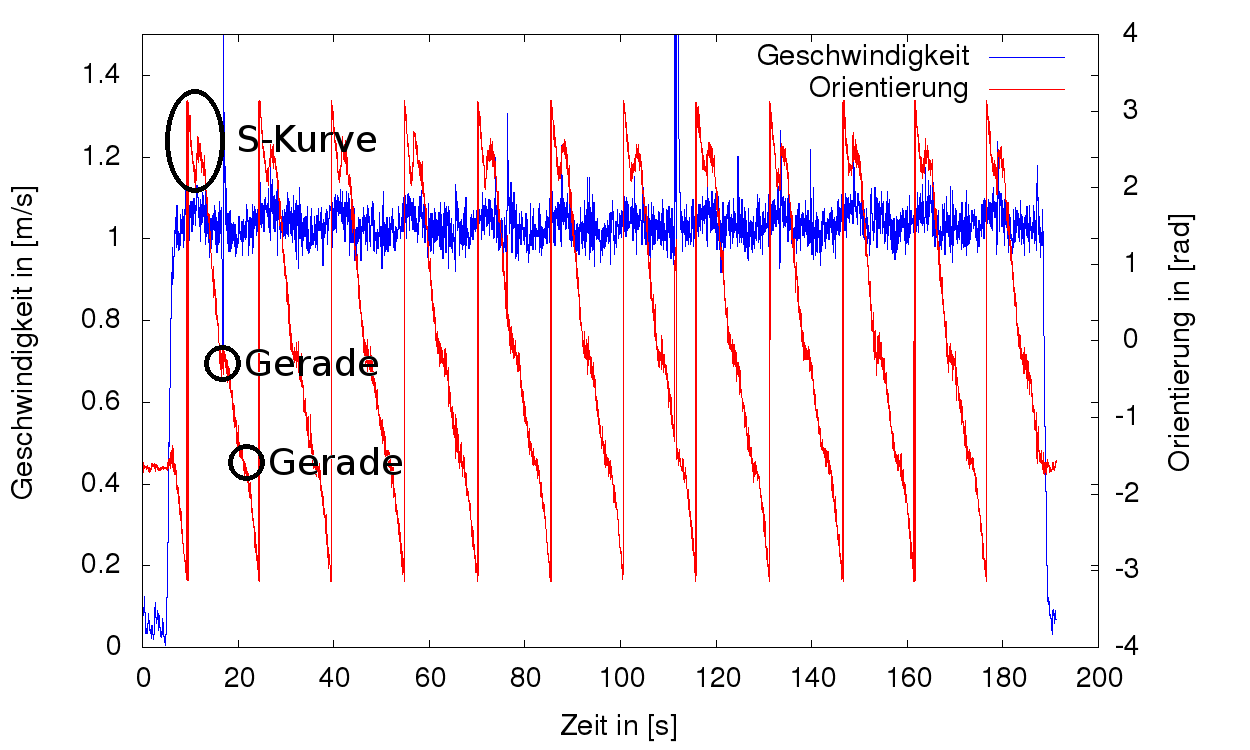
\includegraphics[width=\textwidth]{test.png}\\
\caption{Orientierung und Geschwindigkeit}%
\label{fig:orientation}
\end{figure}


%al type set to 'png'
%Options are 'nocrop enhanced font "Helvetica,20" fontscale 1.0 size 2000,1500 '
%gnuplot> set output "test.png"
%gnuplot> plot 'MessData/odom/test.csv' using 1:2 with line title "Odometrie Geschwindigkeit" axes x1y1, 'MessData/odom/test.csv' using 1:3 with line axes x1y2
%gnuplot> set terminal png size 1200,750 enhanced font "Helvetica,20"
%Terminal type set to 'png'
%Options are 'nocrop enhanced font "Helvetica,20" fontscale 1.0 size 1200,750 '
%gnuplot> set output "test.png"
%gnuplot> plot 'MessData/odom/test.csv' using 1:2 with line title "Odometrie Geschwindigkeit" axes x1y1, 'MessData/odom/test.csv' using 1:3 with line axes x1y2
%gnuplot> set terminal png size 1250,750 enhanced font "Helvetica,20"
%Terminal type set to 'png'
%Options are 'nocrop enhanced font "Helvetica,20" fontscale 1.0 size 1250,750 '
%gnuplot> set terminal png size 1250,750 enhanced font "Helvetica,22"
%Terminal type set to 'png'
%Options are 'nocrop enhanced font "Helvetica,22" fontscale 1.0 size 1250,750 '
%gnuplot> set output "test.png"
%gnuplot> plot 'MessData/odom/test.csv' using 1:2 with line title "Odometrie Geschwindigkeit" axes x1y1, 'MessData/odom/test.csv' using 1:3 with line axes x1y2
%gnuplot> plot 'MessData/odom/test.csv' using 1:2 with line title "Odometrie Geschwindigkeit" axes x1y1 rgb "blue", 'MessData/odom/test.csv' using 1:3 with line axes x1y2 rgb "red"
%
%gnuplot> plot 'MessData/odom/test.csv' using 1:2 with line title "Odometrie Geschwindigkeit" axes x1y1 rgb "blue", 'MessData/odom/test.csv' using 1:3 with line axes x1y2 rgb "red"
%                                                                                                       ^
%         ';' expected%
%
%gnuplot> plot 'MessData/odom/test.csv' using 1:2 with line title "Odometrie Geschwindigkeit" axes x1y1 lt rgb "blue", 'MessData/odom/test.csv' using 1:3 with line axes x1y2 rgb "red"%%
%
%gnuplot> plot 'MessData/odom/test.csv' using 1:2 with line title "Odometrie Geschwindigkeit" axes x1y1 lt rgb "blue", 'MessData/odom/test.csv' using 1:3 with line axes x1y2 rgb "red"
%                                                                                                                                                                             ^
%%         ';' expected%
%
%gnuplot> plot 'MessData/odom/test.csv' using 1:2 with line title "Odometrie Geschwindigkeit" axes x1y1 lt rgb "blue", 'MessData/odom/test.csv' using 1:3 with line axes x1y2 lt rgb "red"
%gnuplot> set output "test.png"
%gnuplot> plot 'MessData/odom/test.csv' using 1:2 with line title "Odometrie" axes x1y1 lt rgb "blue", 'MessData/odom/test.csv' using 1:3 with line title "Tracking" axes x1y2 lt rgb "red"



Während der Datenaufzeichnung fuhr das Fahrzeug den OttoCar-Rund\-kurs ab, es startete  an der Position des Pfeils in dessen Richtung.


\begin{figure}[H]
\centering
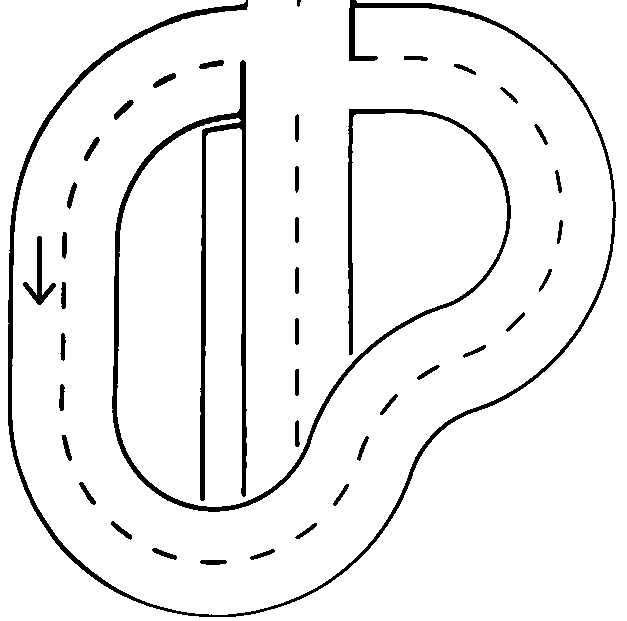
\includegraphics[width=.8\textwidth]{Strasse_mono.png}\\
\caption{OttoCar-Rundkurs}%
\label{fig:strasse}
\end{figure}

Sobald das Auto beschleunigt hat fängt es an seine Orientierung zu ändern. Direkt nach dem 1. Sprung der Orientierung (von -Pi zu Pi)
hat die Geschwindigkeit ihr Maximum. Währenddessen durchfährt das Fahrzeug die S-Kurve des Rundkurses, Der Kurvenradius der S-Kurve ist sehr gering, daher fährt das Fahrzeug
beinahe gerade. Das Fahrzeug scheint also in Kurven bei gleicher Drehzahl langsamer zu fahren, was sich durch  den erhöhten Schlupf in den Kurven erklären lässt. Die Abweichungen 
der Geschwindigkeit in den Kurven ist jedoch sehr gering, sodass diese nur wenig ins Gewicht fallen. Der Wert der Geschwindigkeit ist mit Hilfe des Trackings nicht verifizierbar,
da eine Kalibrierung dessen auf Grund des Entwicklungsstandes nicht erfolgt ist. Das Tracking ist somit als Referenzsystem nicht geeignet, da die zurückgelegte Strecke im vorherigen
Abschnitt jedoch bereits evaluiert wurde ist dies nicht nötig.


\section{Stromverbrauch}

Der Stromverbrauch des Fahrzeugs ist ein wichtiges Kriterium in den statischen Disziplinen. Um den Stromverbrauch im laufenden Betrieb messen zu können, wird hier ein Versuchsaufbau verwendet welcher der Messung des
Motorstromes ähnelt. Die Schaltung besteht dabei aus einem Shuntwiderstand, einer aktiven Filterschaltung und einem Arduino, welcher die Daten zum NUC weiterleitet. Der Vorteil dieser Methode ist, dass die Daten
unter realen Bedingungen in Echtzeit aufgezeichnet werden können. \cref{fig:power_consumption} zeigt den Verlauf der Leistungsaufnahme während folgendem Szenario: Bis ca. \SI{25}{\second} steht das Auto, sämtliche Software, des OttoCar-Projekts (inklusive
der Bildverarbeitung), ist dabei auf 
dem Fahrzeug aktiv. Ab \SI{25}{\second} beschleunigt das Fahrzeug auf \SI{1,3}{\metre\per\second} und verharrt dort bis ca. Sekunde 57, in welcher es gegen eine Wand fährt. Der grüne Graph stellt dabei den Strom durch den Motor dar, während
der blaue Graph den Gesamtverbrauch des Fahrzeugs darstellt. Die roten Linien stellen einen gleitenden Mittelwert aus den letzten 200 Messwerten dar. Gut zu erkennen ist, dass der Stromverbrauch des Fahrzeugs im Stand unter 
\SI{10}{\watt} liegt. Der Mittelwert des Verbrauches im Stand beträgt \SI{7,9}{\watt}, während das Fahrzeug während der Fahrt knapp \SI{13}{\watt} an Leistung aufnimmt. Nur während das Fahrzeug beschleunigt benötigt es für die Dauer
des Beschleunigungsvorganges mehr Leistung. Fährt das Fahrzeug gegen ein Hindernis, sodass die Räder blockieren, befindet sich der Motor im Kurzschlussbetrieb, dabei reduziert sich sein Widerstand auf den Ohmschen Widerstand
des Motors, was zu einem hohen Stromfluss durch den Motor führt. Dauerhaft kann das durch Überhitzung zur Zerstörung des Motors oder der Treiberplatine führen.

\begin{figure}[H]
\centering
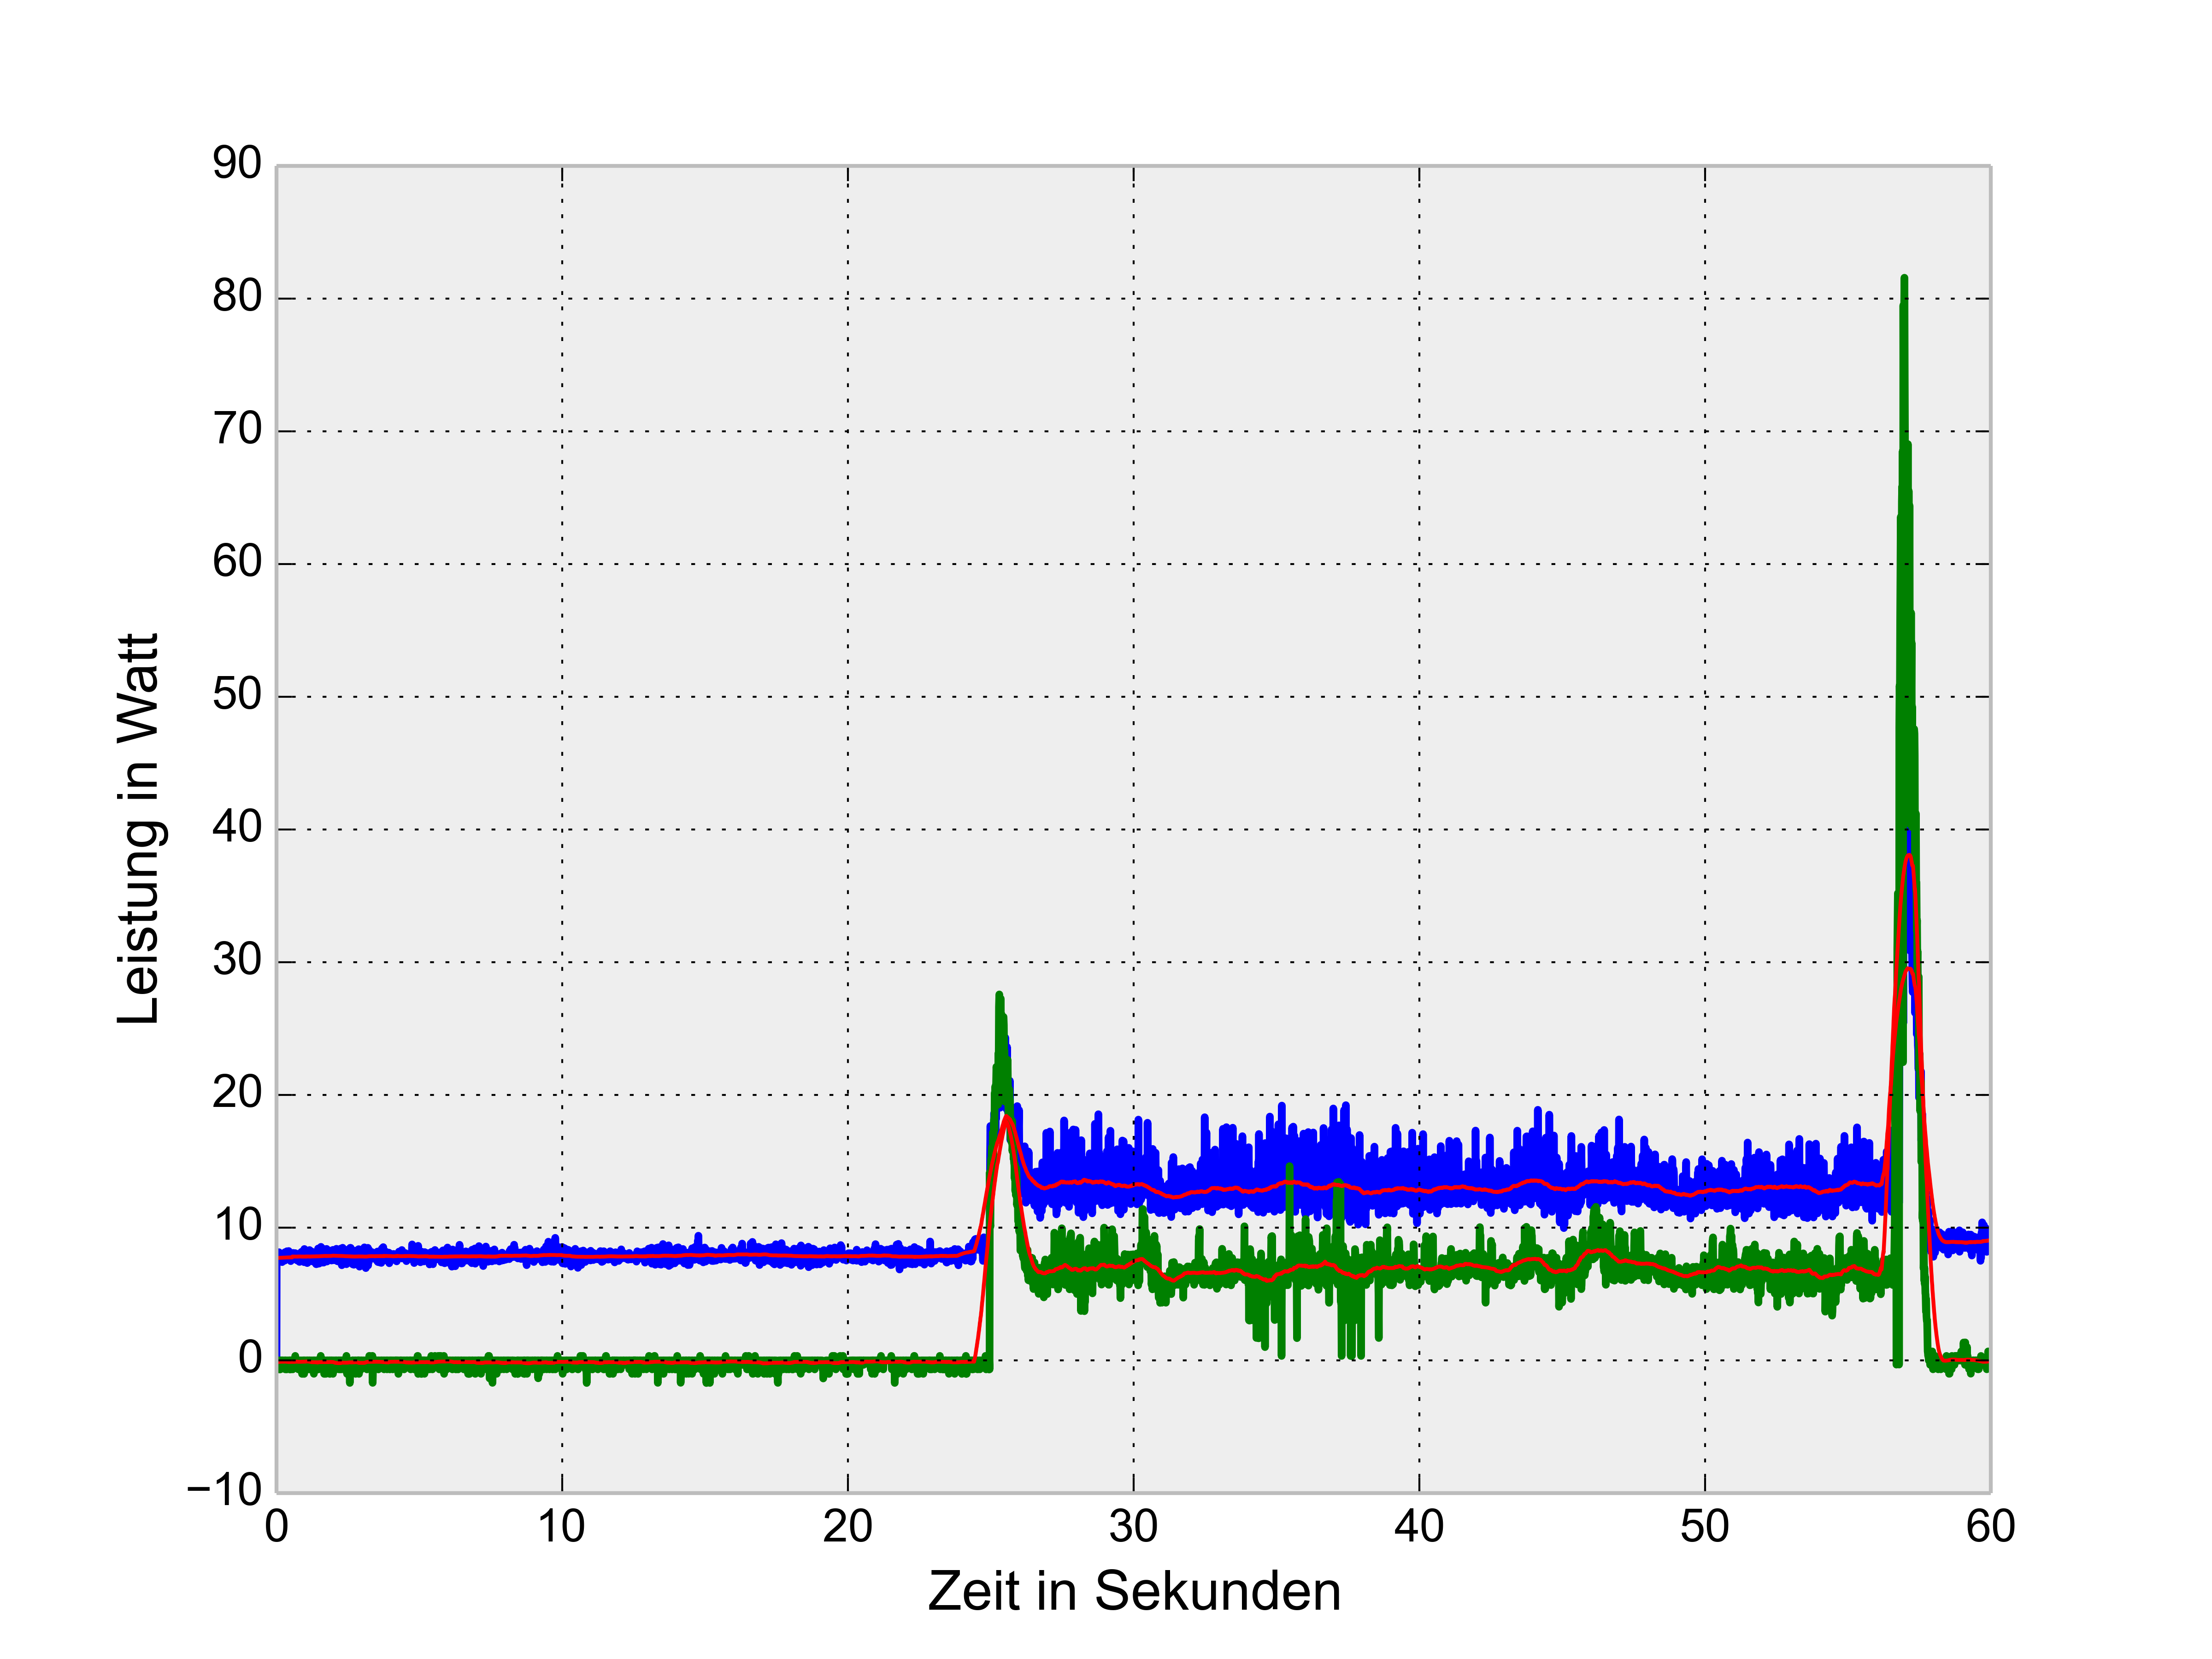
\includegraphics[width=.8\textwidth]{Strom/Power.png}\\
\caption{Stromverbrauch des Fahrzeuges}%
\label{fig:power_consumption}
\end{figure}

Die starken Schwankungen der Messwerte werden durch die vor den Akku geschaltete Strommessung verursacht. Der Shuntwiderstand in dieser Schaltung hat eine Größe von
\SI{0,2}{\ohm}, was den Innenwiderstand der Akkus stark erhöht und dadurch die Spannungsschwankungen der Betriebsspannung verstärkt. 

\subsection{Vergleich der Motormodi}
Im folgenden werden zwei Motormodi miteinander verglichen, und zwar  \{PWML=1, PHASE=1, SR=0\} und  \{PWML=1, PHASE=1, SR=1\} jeweils nur mit high-side PWM.


\subsubsection{Stromverbrauch \{PWML=1, PHASE=1, SR=1\}}

In \cref{fig:power_consumption_sr} lässt sich wieder gut der erhöhte Stromverbrauch beim Anfahren von Sekunde 1 bis 3 erkennen, das Fahrzeug beschleunigt in dieser Zeit
von \SI{0}{\metre\per\second} auf \SI{1}{\metre\per\second}. Der Bremsstrom des Motor kann in diesem Modus nahezu ungestört durch die Mosfets fließen, da diese einen
sehr niedrigen Widerstand aufweisen (ca. \SI{12}{\mohm}). Dadurch beleibt das Fahrzeug nach der Reduzierung des Tastgrades auf 0:256 bereits nach weniger als \SI{10}{cm} zum stehen.

\begin{figure}[H]
\centering
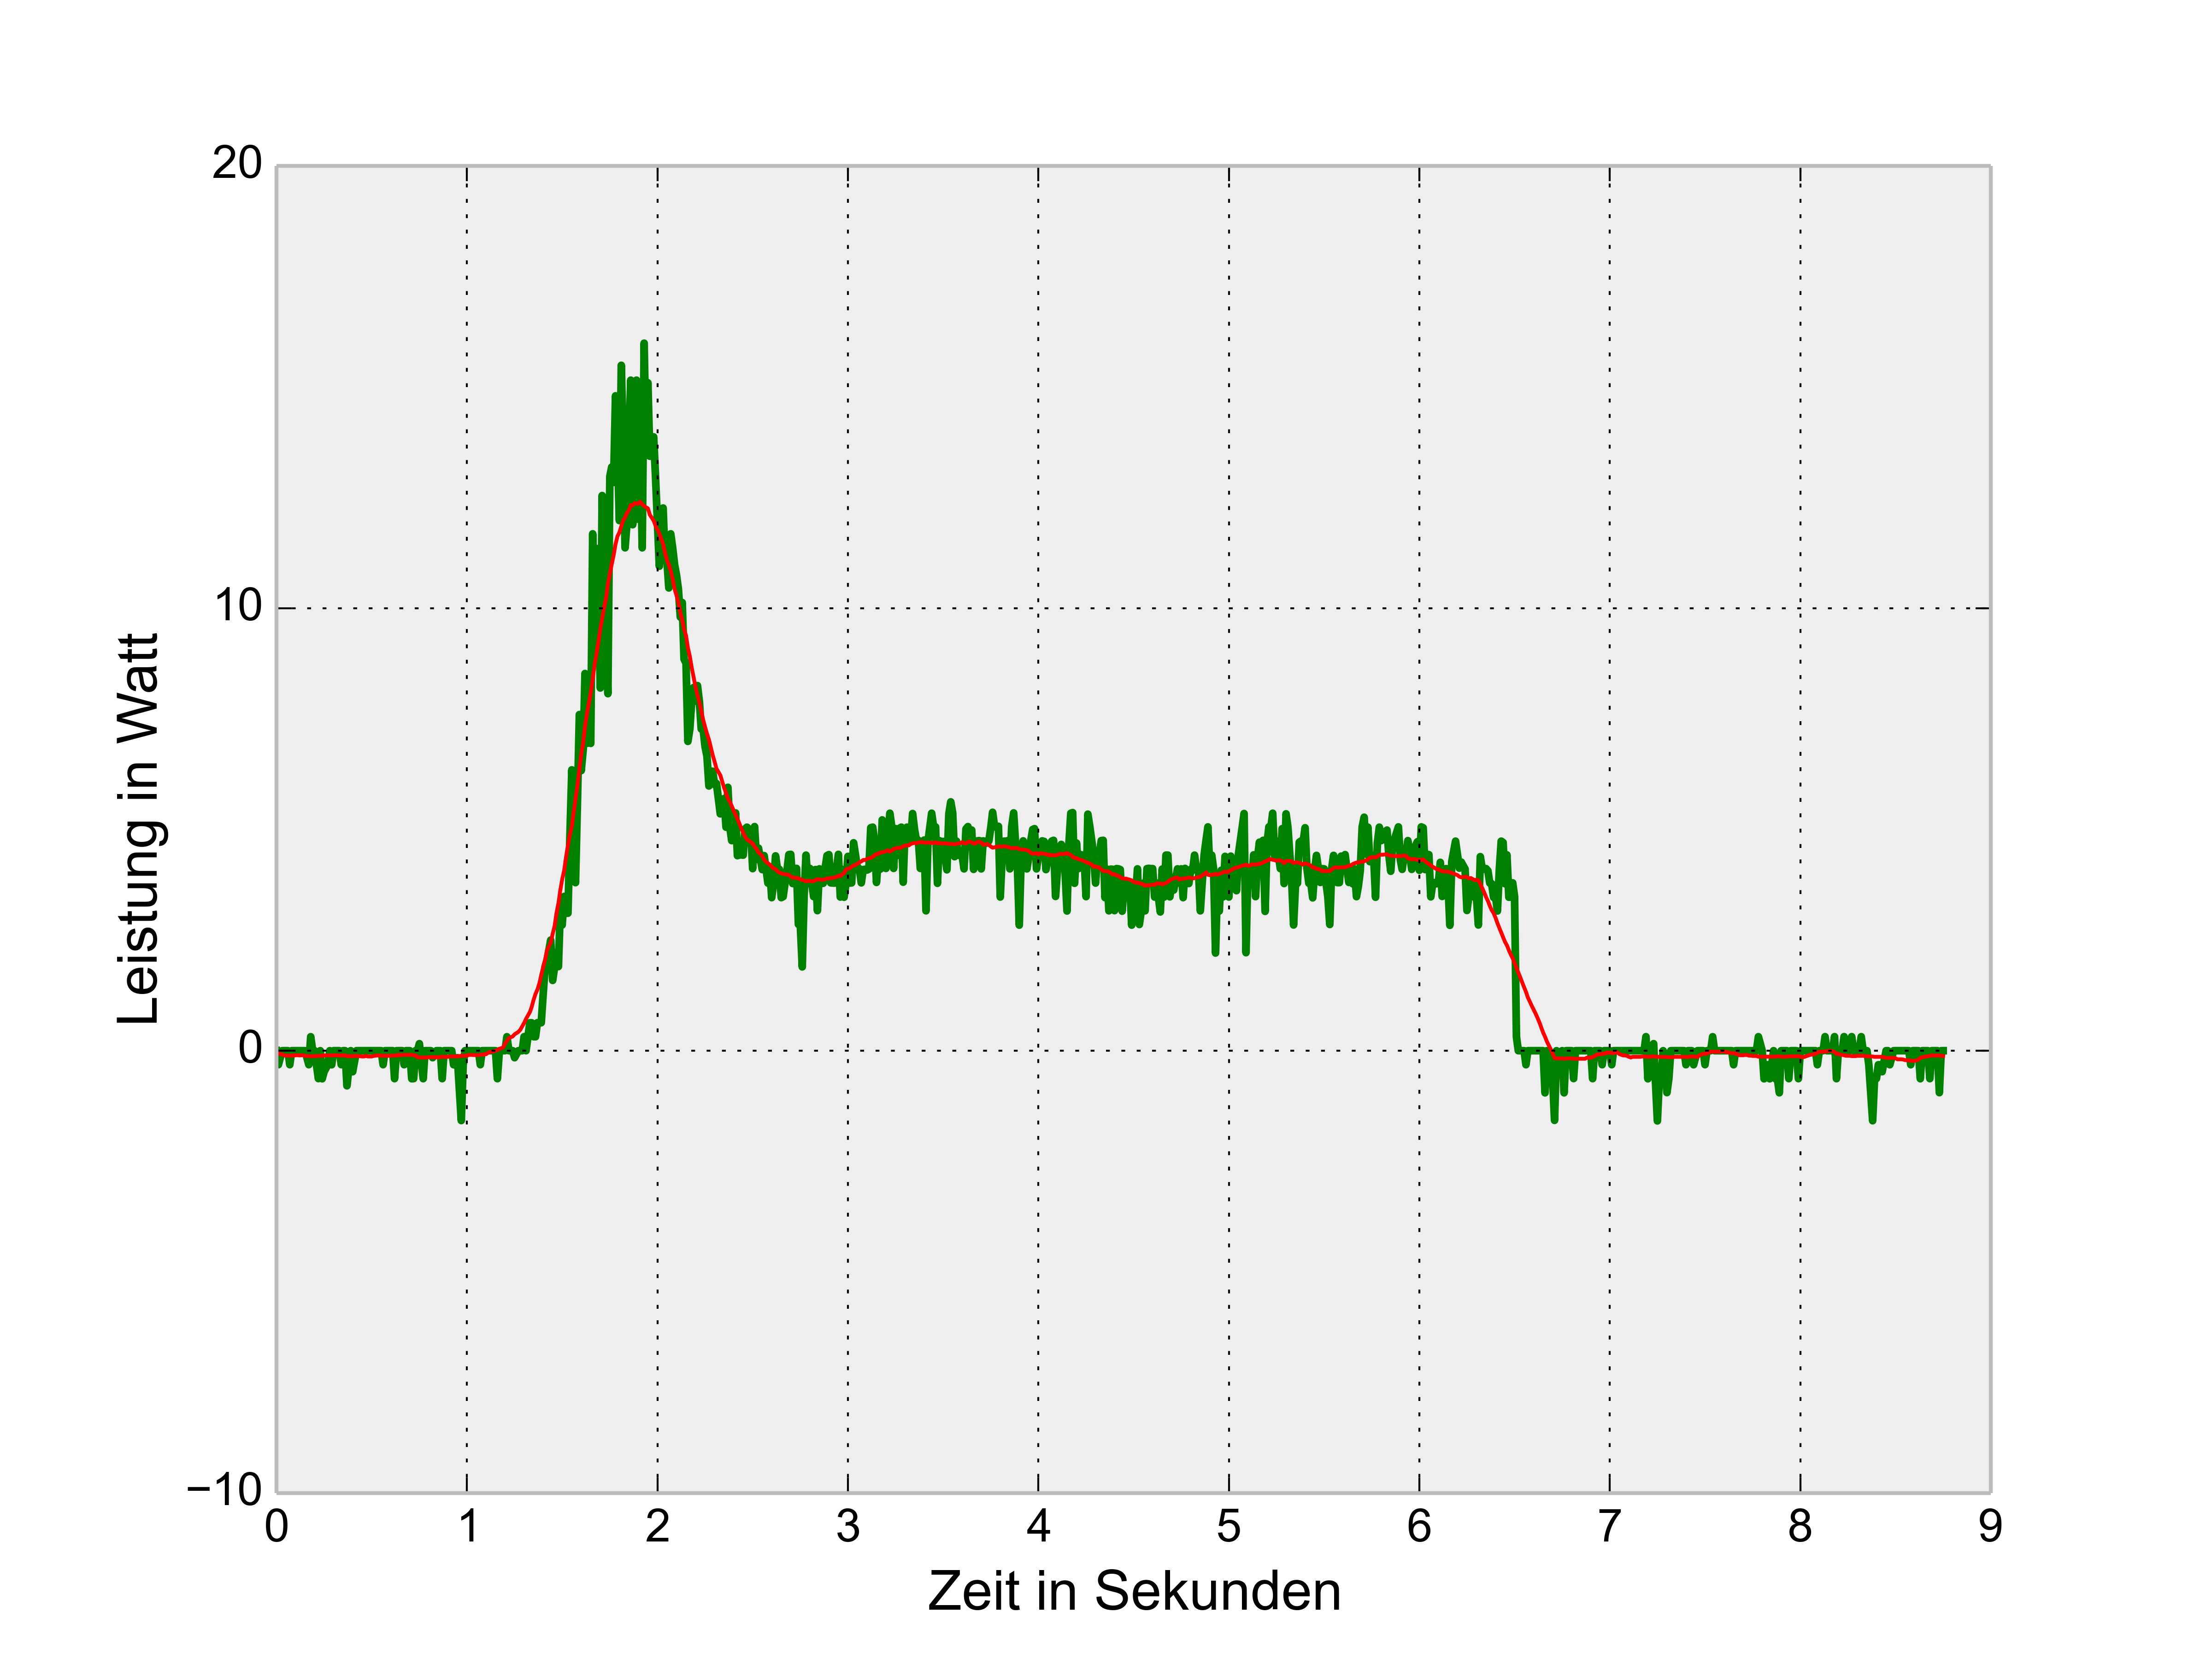
\includegraphics[width=.8\textwidth]{Strom/sr_power.png}\\
\caption{Stromverbrauch des Fahrzeuges mit SR}%
\label{fig:power_consumption_sr}
\end{figure}

Der Mittelwert des Stromverbrauchs liegt im konstanten Fahrbetrieb bei \SI{4,24}{\W}.

\subsubsection{Stromverbrauch \{PWML=1, PHASE=1, SR=0\}}


In \cref{fig:power_consumption_nsr} lässt sich ebenfalls gut der erhöhte Stromverbrauch beim Anfahren von Sekunde 1 bis 3 erkennen, das Fahrzeug beschleunigt in dieser Zeit wieder
von \SI{0}{\metre\per\second} auf \SI{1}{\metre\per\second}. Da der Bremsstrom in diesem Motor durch die internen Dioden der Mosfets fließt und dadurch kleiner als im
voherigen Fall ist. Rollt das Fahrzeug trotz einem Tastgrad von 0:256 ca. \SI{50}{\cm} weiter.


\begin{figure}[H]
\centering
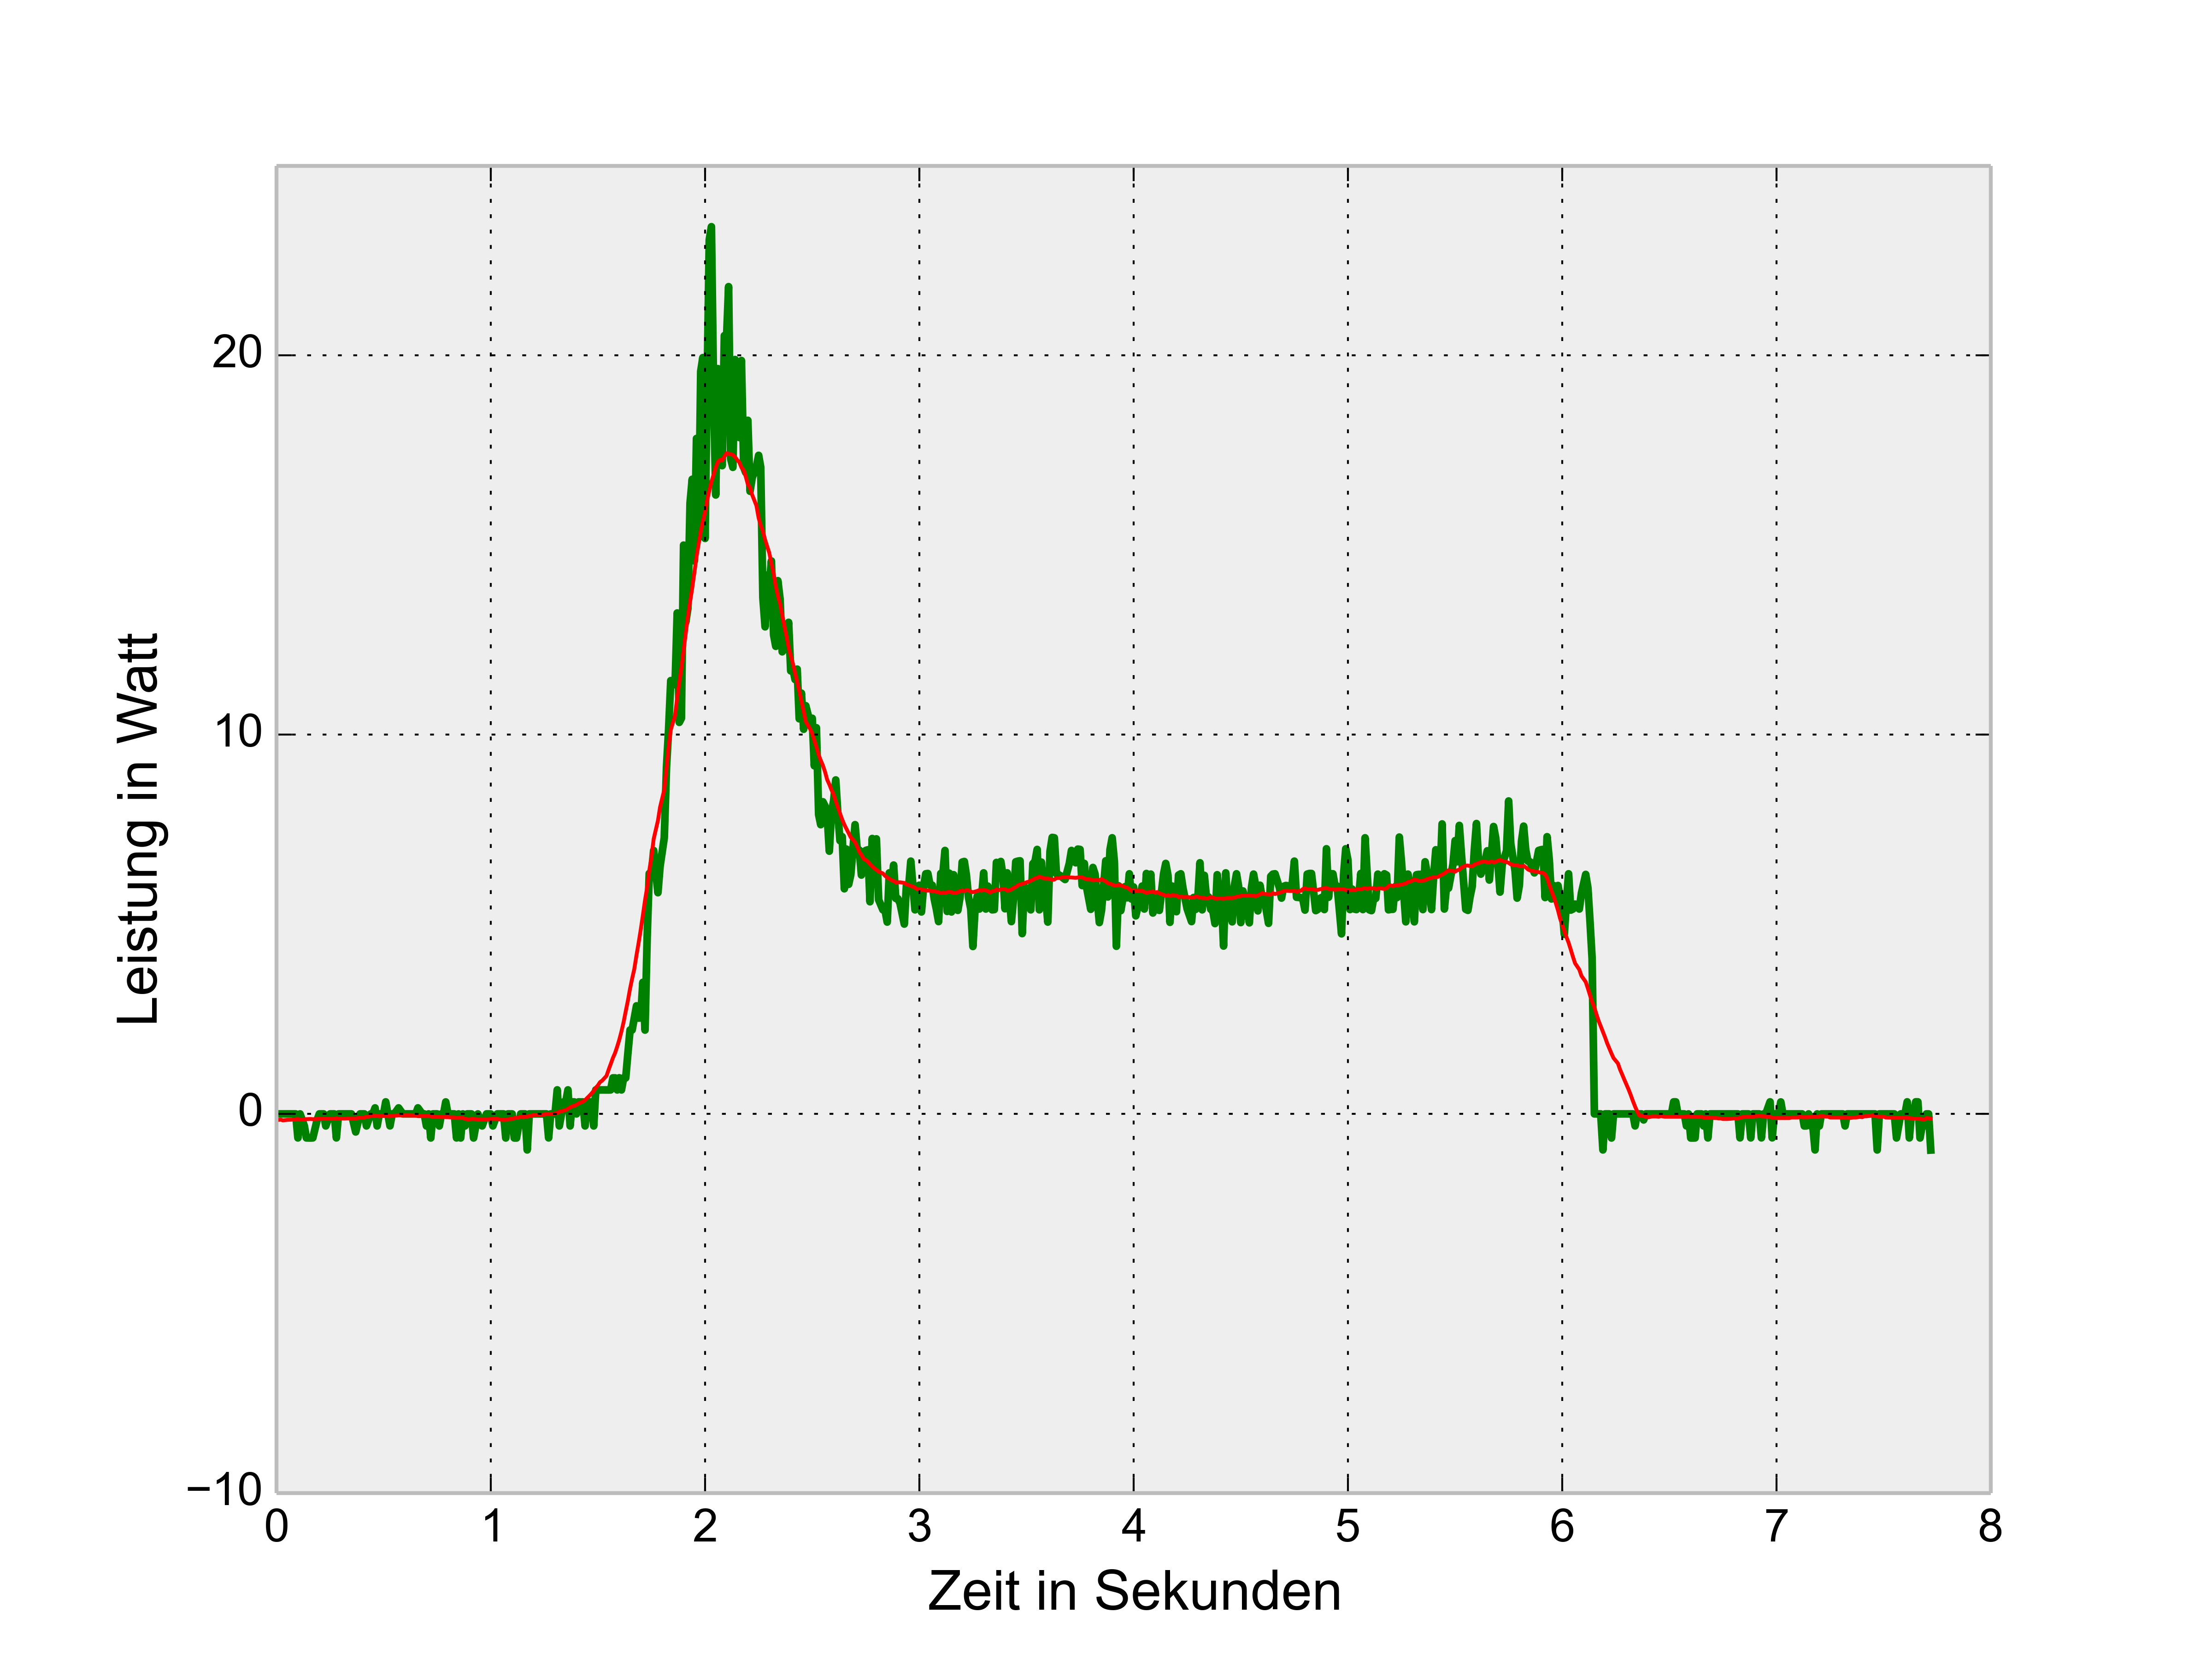
\includegraphics[width=.8\textwidth]{Strom/nsr_power.png}\\
\caption{Stromverbrauch des Fahrzeuges ohne SR}%
\label{fig:power_consumption_nsr}
\end{figure}

Der Mittelwert des Stromverbrauchs liegt im konstanten Fahrbetrieb bei \SI{5,13}{\W}.

Der Modus mit SR ist dem Modus ohne SR vorzuziehen, zum einen ist der Verbrauch in den Messungen durchgängig besser, zum anderen erlaubt der SR-Modus eine bessere Fahrzeugkontrolle.
Durch die stärkere Bremswirkung im SR-Modus spricht das Auto besonders gut auf einen Geschwindigkeitswechsel an.

\subsection{Vergleich innerhalb des „Carolo-Cup“}
Ein direkter Vergleich des Stromverbrauchs mit anderen Teams des vergangenden „Carolo-Cup“ 2014 ist leider kaum möglich, da in den vorhandenen Quellen (Teampräsentationen) nur sehr selten
angaben über die Bedingungen der Messung gemacht werden. Die Angaben variieren dabei von \SI{10}{\W} (Berlin-United-Racing Team \cite{cc-bu}) bis zu \SI{161}{\W}(Team CDLC \cite{cc-cdlc}).
Team ``Tetrix''\cite{cc-tx} gibt ihren Stromverbrauch jedoch mit \SI{66,2}{\W} bei \SI{1}{\metre\per\second} und ist somit das einzige vergleichbare Team. Von diesem Wert entfallen
laut der Präsentation \SI{47}{\W} auf den Motor. Dieser Wert scheint jedoch viel zu hoch, so dass hier von einer Fehlerhaften Messung des Team ``Tetrix'' ausgegangen wird.

